\documentclass[../main.tex]{subfiles}
\graphicspath{{\subfix{../Images/}}}
\begin{document}

\section{Sensor Calibration} \label{sec:calibration}

The multi-sensor perception suite described in the previous section integrates complementary sensing modalities: \ac{LiDAR} for spatial structure and cameras for visual context.
Each of these sensors measures the environment within its own local reference frame and according to its own internal clock.
To combine their observations into a consistent world model, the system must first be calibrated both spatially and temporally.
% Target calibration accuracy for the Minion platform was defined as less than $1^{\circ}$ rotational error, less than 1~cm translational error, and no more than 20~ms temporal offset across all sensors.

For the Minion platform, all sensors are rigidly mounted and assigned reference frames within a unified transform hierarchy. 
The GPS receiver anchors the global \texttt{map} frame; the ROS TF tree (Fig.~\ref{fig:tf_tree}) resolves transforms such as \texttt{map}\ $\rightarrow$\ \texttt{base\_link} and \texttt{base\_link}\ $\rightarrow$\ \texttt{sensor}. Spatial calibration estimates the rigid rotations and translations that populate this tree.  
Intrinsic calibration is also required for the visible-spectrum cameras (shown in blue), determining the internal optical parameters such as focal length, principal point location, and lens distortion. 
Time synchronization is similarly structured, with a master clock distributed over the network to subsystems and sensors to ensure that data acquired across sensor modalities remain temporally aligned.

% Within this framework, the port and starboard Livox units are first registered to the center Livox reference frame, where their point clouds are merged into a single unified point cloud.  
% This consolidated LiDAR frame is then related to the HDR camera world-frame through an additional extrinsic transform and finally to the camera's image-frame through the determined camera intrinsic values, allowing three-dimensional LiDAR points $(x, y, z)$ to be projected onto the two-dimensional image plane $(u, v)$ using the camera’s intrinsic parameters.  
% Finally, all perception data are kept in sync and expressed in the global map frame defined through the time, location, and orientation provided by the \ac{GPS}.
Within this framework, the port and starboard Livox units are first registered to the center Livox reference frame to produce a unified point cloud. 
The consolidated LiDAR frame is then related to the HDR camera world frame through an additional extrinsic transform. 
Using the camera’s intrinsic parameters, three-dimensional LiDAR points $(x, y, z)$ can then be projected onto the two-dimensional image plane and expressed as pixel locations $(u, v)$. 
An additional series of extrinsic transforms relates the central Livox frame to the \ac{GPS} antenna frame, and the \ac{GPS} frame to the global map frame. 
The \ac{GPS} provides dual functionality, maintaining synchronization across all sensor data and orienting them within the static global map frame.

% All perception data are synchronized and expressed in the global map frame, defined by the time, location, and orientation provided by the \ac{GPS}.

An initial calibration of the camera enclosure was performed during earlier work by Thompson~\cite{thompson2023}, establishing the baseline intrinsic camera parameters and the extrinsic relationship between the three Livox LiDAR units.
In the multiple years between data collection campaigns, the camera enclosure was relocated multiple times and subjected to extended periods of vibration during transport of the \ac{USV} on its trailer.
These mechanical stresses alone were sufficient to warrant recalibration, as small shifts in sensor mounts or camera optics can accumulate over time and degrade geometric alignment.
Compounding this, the center Livox unit suffered a hardware failure and was replaced, making a full recalibration of all extrinsic transforms essential before further data collection.

Section \ref{spatial_calibration} provides the methods used for intrinsic camera calibration, extrinsic calibration between the camera and LiDAR sensors, and between the individual LiDAR units. 
This is followed by a discussion of the time synchronization methods implemented across the network, with special detail provided to the timestamps applied to video frames in section \ref{time_sync}
Finally, the resulting spatial calibration accuracy and temporal alignment obtained are discussed in section \ref{time_sync}.



\begin{figure}[htbp]
    \centering
    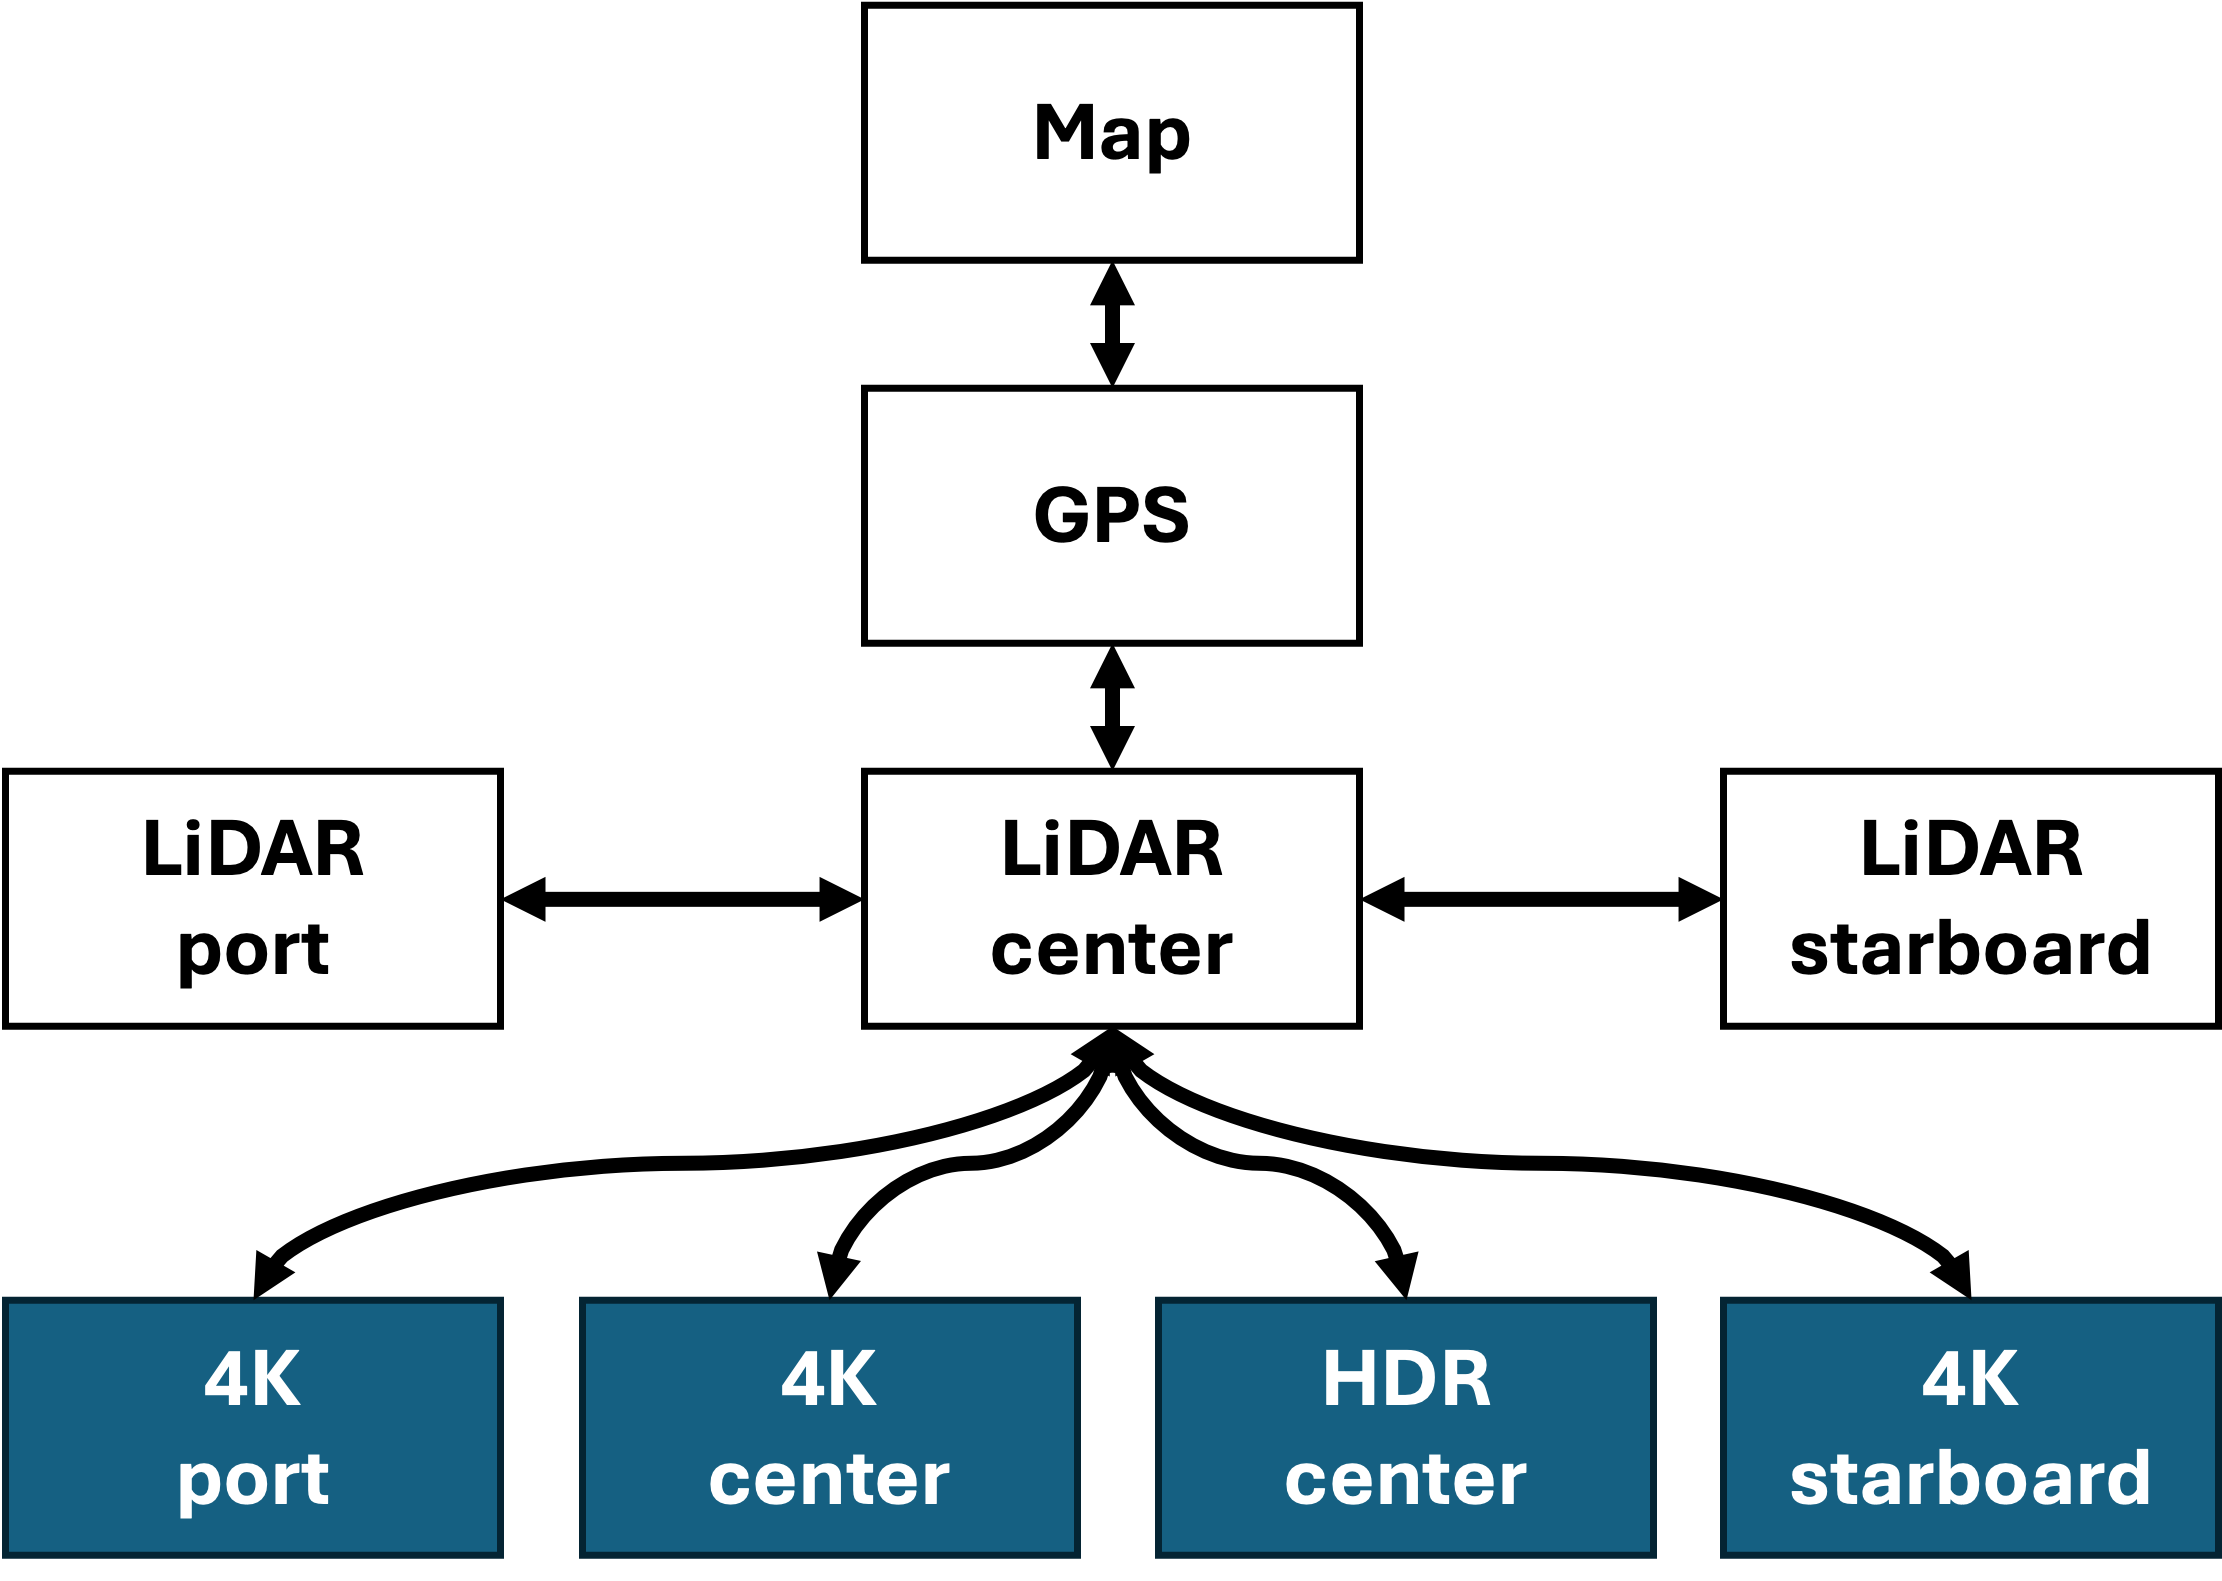
\includegraphics[width=0.7\linewidth]{Images/tf_tree_1.png}
    \caption{Transform hierarchy for Minion: the GPS-defined \texttt{map} frame anchors the ROS TF tree used for LiDAR–camera projection and sensor fusion.}
    \label{fig:tf_tree}
\end{figure}

%%%%%%%%%%%%%%%%%%%%%%%%%%%%%%%%%%%%%%%%%%%%%%%%%%%%%%%%%%%%%%%%%%%%
\subsection{Spatial Calibration} \label{spatial_calibration}

Before data from the camera and \ac{LiDAR} sensors can be combined, each device must be spatially calibrated through intrinsic and extrinsic transformations.  
This process establishes the geometric relationships required to express all sensor measurements in a unified coordinate frame, enabling accurate projection of \ac{LiDAR} points onto the camera image plane.

Calibration begins with determining the camera’s intrinsic parameters, followed by estimation of the extrinsic transformation that defines the rigid-body relationship between the camera and each \ac{LiDAR} sensor.  
The following sections describe the methods and results of this calibration process.

%%%%%%%%%%%%%%%%%%%%%%%%%%%%
\subsubsection{Extrinsic Calibration} \label{extrinsic_tform}

Extrinsic calibration defines the rigid-body transformation between two reference frames.  

The transformation from frame $A$ to frame $B$ is represented as
\begin{equation}
    _{B}^{A}\mathbf{T} =
    \begin{bmatrix}
        _{B}^{A}\mathbf{R} & _{B}^{A}\mathbf{t} \\
        \mathbf{0}^\mathrm{T} & 1
    \end{bmatrix},
\end{equation}

where $\mathbf{R}_{B}^{A} \in \mathbb{R}^{3\times3}$ is the rotation matrix describing the orientation of frame $A$ relative to frame $B$, and $_{B}^{A}\mathbf{t} \in \mathbb{R}^{3}$ is the translation vector locating the origin of frame $A$ with respect to frame $B$.  
The notation convention used here is that the subscript denotes the destination frame and the superscript the source frame.

A point $_{A}\mathbf{P}$ expressed in frame $A$ can therefore be transformed into frame $B$ as

\begin{equation}
    _{B}\mathbf{P} =
    _{B}^{A}\mathbf{R} _{A}\mathbf{P} + _{B}^{A}\mathbf{t}.
\end{equation}

This formulation provides a consistent framework for representing spatial relationships among all platform sensors.  
Transformations can be sequentially composed through the transform tree shown in Figure~\ref{fig:tf_tree}, allowing points measured by any sensor to be expressed in a common reference frame and projected into the camera image for spatial alignment.

The \ac{LiDAR}-to-\ac{LiDAR} extrinsic calibration defines the rigid-body transformations relating the three Livox Horizon units to a shared coordinate system.  
The center unit serves as the reference frame, with the port and starboard sensors calibrated relative to it to create a unified, geometrically consistent point cloud.

Using large flat surfaces such as walls or other well-defined objects within the unit's overlapping field of view allows the sensors to be aligned.
The Livox devices used have a functional detection range of 260~m \cite{livox_manual}, which is far greater than the intended operational range for the sensor fusion presented in this research. 
Due to the divergent nature of the scanning pattern, a simple visual inspection  (as illustrated in figure \ref{fig:Lidar2Lidar}) of sensor alignment beyond 100~m guarantees alignment at closer range. 

\begin{figure}[htbp]
    \centering
    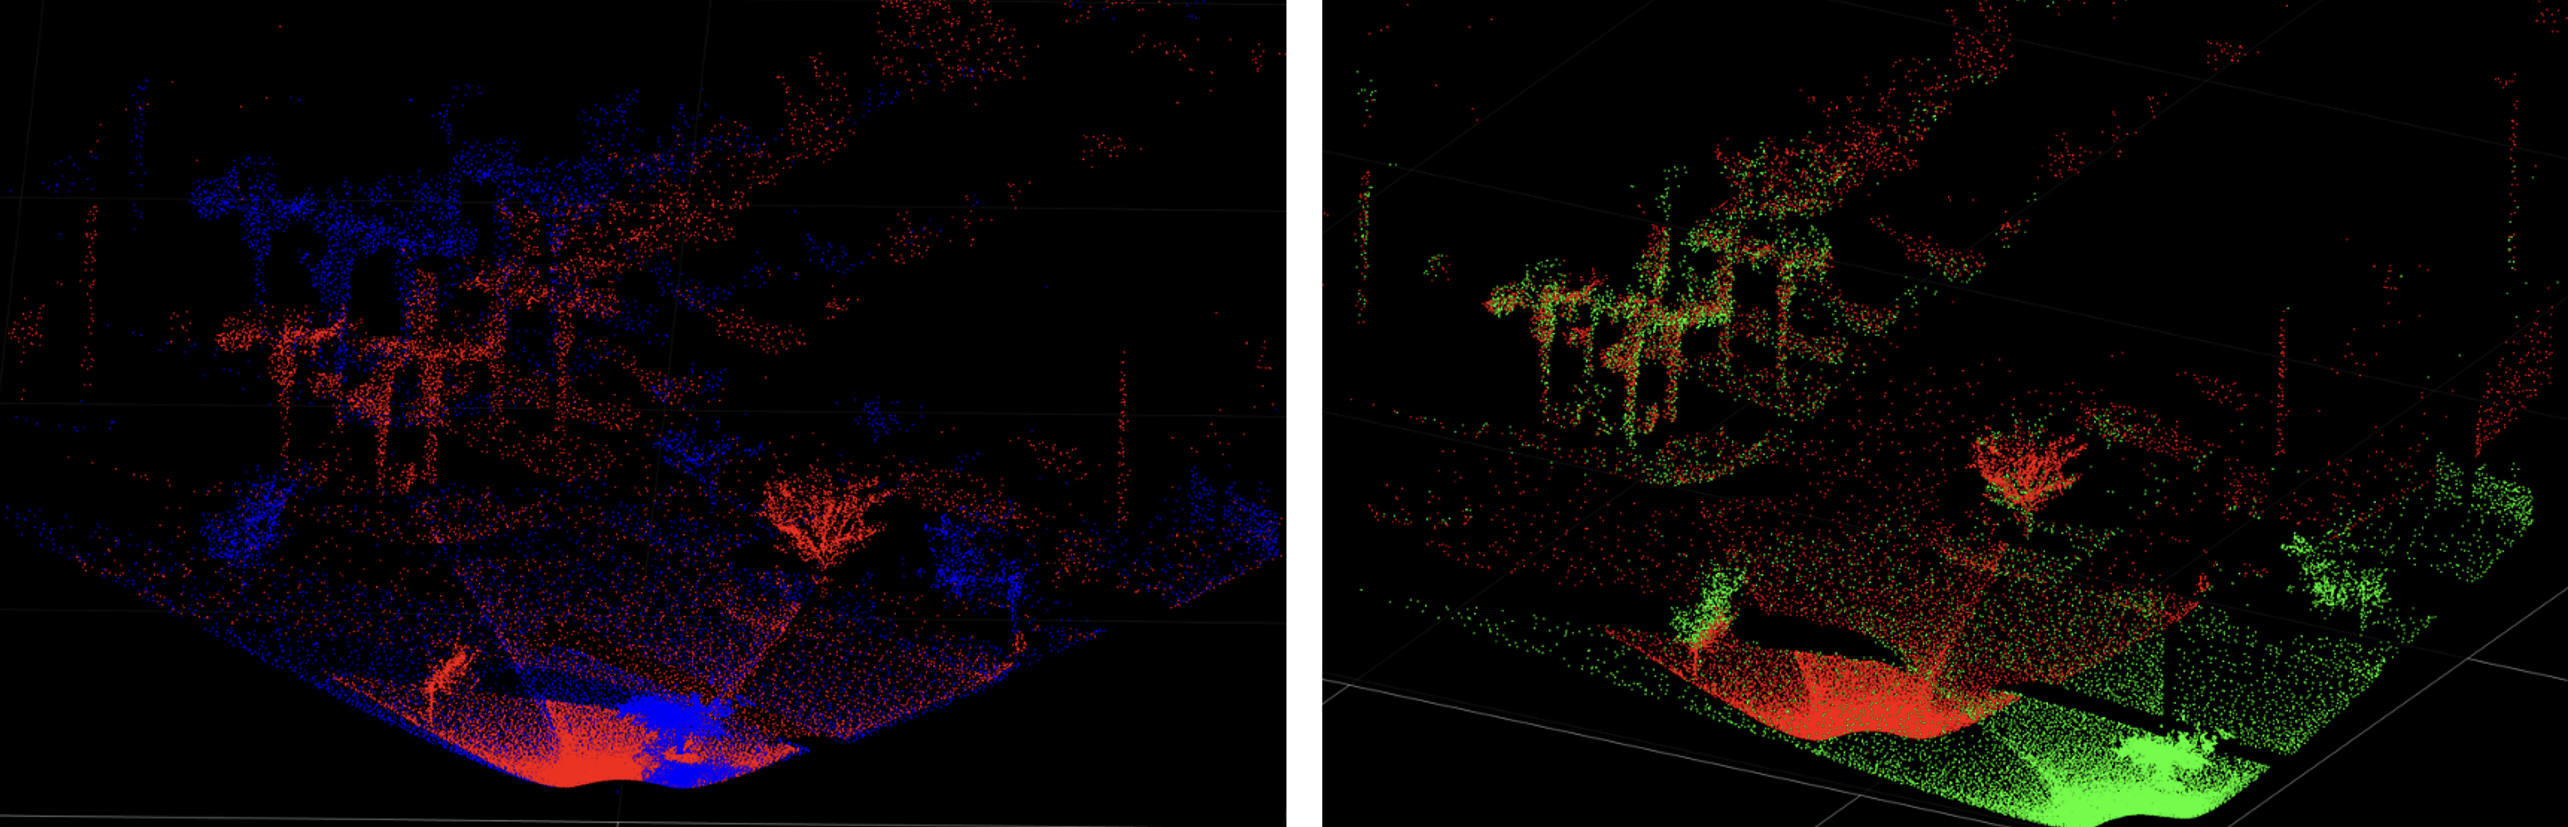
\includegraphics[width=0.9\linewidth]{Images/Lidar2Lidar.png}
    \caption{Example of LiDAR–LiDAR alignment.}
    \label{fig:Lidar2Lidar}
\end{figure}

%%%%%%%%%%%%%%%%%%%%%%%%%%%%
\subsubsection{Camera Intrinsics} \label{camera_intrinsics}

Camera intrinsic parameters describe the internal geometry of the camera and define how three-dimensional points are projected onto the two-dimensional image plane.  
They are governed by the optical pathway through the lens and determine how real-world distances correspond to image pixel coordinates.  
The intrinsic model is typically divided into an idealized pinhole projection and a lens distortion model.

Under the pinhole model, the projection of a point onto the image plane is given by the intrinsic matrix:

\begin{equation}
    \mathbf{K} = 
    \begin{bmatrix}
        f_x & s & c_x \\
        0 & f_y & c_y \\
        0 & 0 & 1
    \end{bmatrix},
\end{equation}

where $(f_x, f_y)$ are focal lengths in pixels, $(c_x, c_y)$ denotes the principal point, and $s$ represents the skew factor (generally $s=0$ for modern sensors).

Real lenses introduce distortion, primarily radial, due to refraction near the outer edge of the lens.  
This effect, most pronounced in wide-angle optics, causes straight lines to appear curved.  
Radial distortion is modeled using polynomial coefficients $k_1$, $k_2$, and $k_3$:
\begin{equation}
    \begin{split}
        x' &= x_n(1 + k_1 r^2 + k_2 r^4 + k_3 r^6), \\
        y' &= y_n(1 + k_1 r^2 + k_2 r^4 + k_3 r^6),
    \end{split}
\end{equation}

where $(x', y')$ are distorted coordinates, $(x_n, y_n)$ are ideal coordinates, and $r = \sqrt{x_n^2 + y_n^2}$ is the radial distance from the optical center.  
Although this model omits asymmetric distortions, high-quality lenses typically minimize such effects.  
Even with manufacturer-provided parameters, recalibration ensures sub-pixel accuracy when aligning \ac{LiDAR} projections with image data.

To estimate intrinsic parameters, a planar checkerboard with known square dimensions is imaged from multiple orientations and distances.  
Its grid of high-contrast corners serves as stable reference points for gradient-based corner detection algorithms such as the Harris method.  
Calibration software uses these detected points to compute statistically optimal parameters across the full image set.

Effective calibration requires dozens of images taken at diverse depths and orientations spanning the camera’s operational field of view.  
Checkerboard dimensions should approximate the scale of observed objects to ensure that the chosen camera provides adequate spatial resolution (as discussed in Section~\ref{camera_selection}).  
Following these practices produces robust intrinsic estimates across the full imaging range.

\begin{figure}[htbp]
\centering
\makebox[\textwidth][c]{%
    \begin{subfigure}[t]{0.3\textwidth}
        \centering
        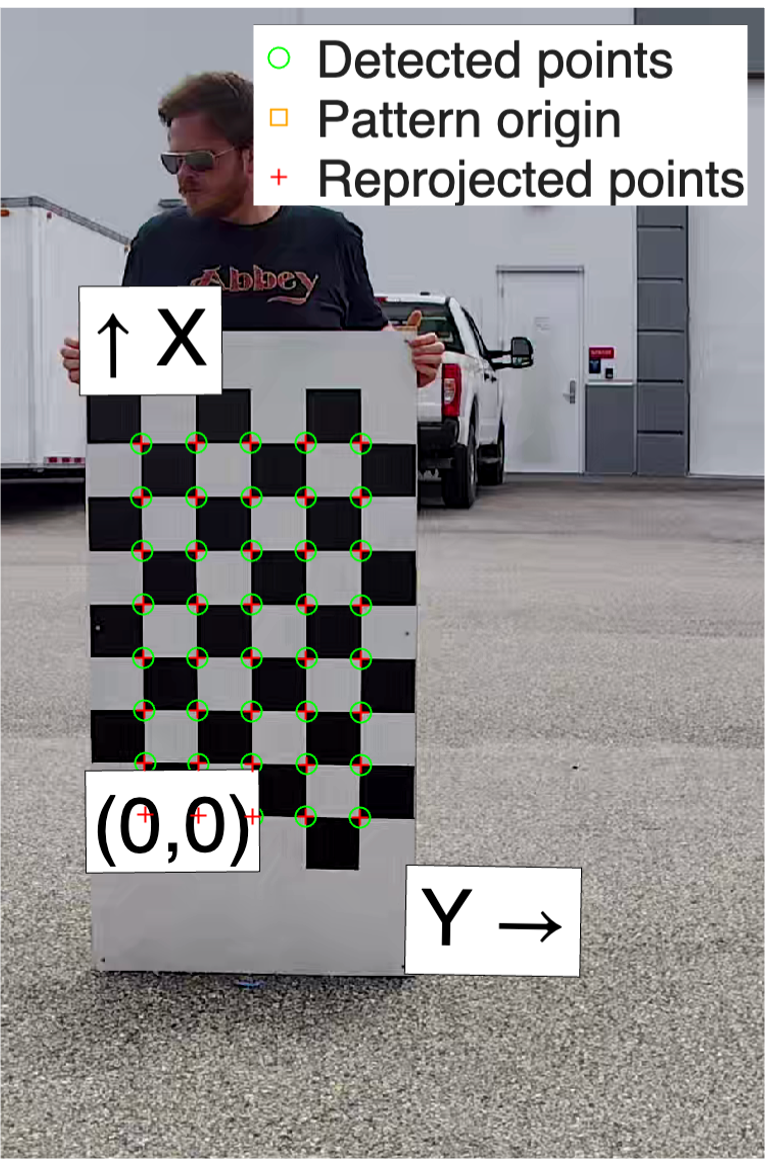
\includegraphics[width=\textwidth]{Images/cam_calib_1.png}
        \caption{A single example of detected and reprojected checkerboard corners. Agreement between detected (green circles) and reprojected (red crosses) points demonstrates corner localization and mapping of the image coordinate system.}
        \label{fig:cam_calib_1}
    \end{subfigure}
    \hspace{2em}
    \begin{subfigure}[t]{0.625\textwidth}
        \centering
        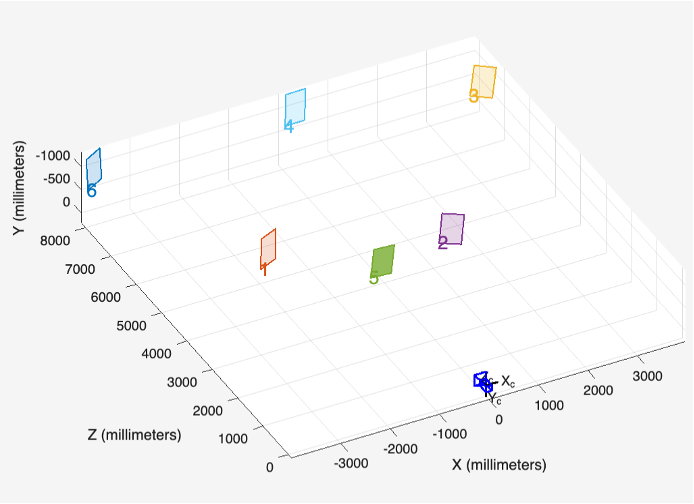
\includegraphics[width=\textwidth]{Images/cam_calib_2.png}
        \caption{Reprojection of sample target poses into the 3D world frame after calibration.}
        \label{fig:cam_calib_2}
    \end{subfigure}%
}
\caption{Checkerboard images are processed to detect corners (left), which enable intrinsic parameters to be estimated and validated by reprojecting known targets into 3D space (right).}
\label{fig:cam_calib}
\end{figure}


%%%%%%%%%%%%%%%%%%%%%%%%%%%%
\subsubsection{Camera to LiDAR Extrinsic Calibration} \label{camLidar_calib}

Camera–LiDAR calibration begins by positioning a planar checkerboard target within both the LiDAR field of view and the camera image.  
The target’s physical dimensions in the LiDAR frame $(X_L, Y_L, Z_L)$ are matched to corresponding pixel coordinates $(u,v)$ in the image, yielding an initial estimate of the rigid transformation between sensor frames.  
A full derivation of this mapping is given in Appendix~\ref{img_tform}, and an example is shown in Figure~\ref{fig:calib_check}.

Initial calibration is performed using software such as the MATLAB LiDAR Calibration tool \cite{matlab_calibration}.  
Further refinement can be achieved either through iterative manual adjustment or by applying an \ac{ICP} algorithm, which minimizes point-to-plane error between the LiDAR point cloud and the camera-projected checkerboard corners.  
This approach produces a coarse transformation $_{C}^{L}\mathbf{T}$ adequate for accurate projection of LiDAR points into the image frame.

Manual fine-tuning may then be conducted by aligning prominent environmental features—such as walls, trees, and fences—visible in both modalities.  
This visual refinement yields sub-degree rotational and centimeter-level translational precision, sufficient for high-accuracy sensor fusion and object-detection tasks.  
In some cases, minor adjustments to the camera intrinsics are also necessary to compensate for small propagated errors.

\begin{figure}[htbp]
\centering
\makebox[\textwidth][c]{
    \begin{subfigure}[t]{0.44\textwidth}
        \centering
        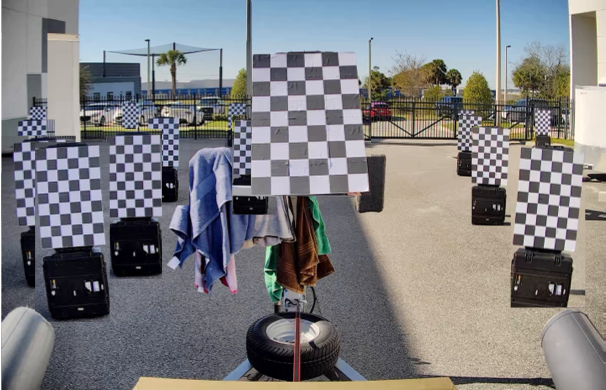
\includegraphics[width=\textwidth]{Images/checkerboard.png}
        \caption{Composite image of multiple checkerboard target locations.}
        \label{fig:checkerboard}
    \end{subfigure}
    \hspace{2em}
    \begin{subfigure}[t]{0.44\textwidth}
        \centering
        \includegraphics[width=\textwidth]{Images/LiDAR_calib.png}
        \caption{Composite of checkerboard locations in the LiDAR reference frame.}
        \label{fig:LiDAR_calib}
    \end{subfigure}
}
\caption{Checkerboard targets used for camera intrinsic (left) and LiDAR extrinsic (right) calibration. Red dots mark detected corner points transformed into the LiDAR frame using the initial extrinsic estimate.}
\label{fig:camLidar_calib}
\end{figure}


%%%%%%%%%%%%%%%%%%%%%%%%%%%%%%%%%%%%%%%%%%%%%%%%%%%%%%%%%%%%%%%%%%%%
\subsection{Results: Spatial Calibration}
\label{sec:spatial_calib_results}
%%%%%%%%%%%%%%%%%%%%%%%%%%%%
\subsubsection{LiDAR–LiDAR Calibration} \label{results_lidarLidar_calib}

% Calibration was performed using the manufacturer’s Livox Viewer software, which provides real-time point cloud visualization and the ability to view, modify, and store sensor extrinsic measurements on-device.
% This interface enables manual adjustment and fine-tuning to minimize misalignment across large planar surfaces such as walls.  
% Once optimal alignment is achieved, the extrinsic parameters can be stored in each sensor’s onboard memory.
% The port and starboard Livox units use this information to transform the data into the central Livox frame prior to transmission, reducing the computational load on Atlas. 

Calibration was performed using the Livox Viewer software, which provides real-time multi-sensor point cloud visualization and tools for automatic calibration and manual adjustment of extrinsic parameters (as shown in Figure~\ref{fig:LidarLidar_calib}). 
The calibration process involved fine-tuning of the $x, y, z$ distance and roll, pitch, and yaw between sensors.
% until a consistent alignment was achieved across overlapping fields of view, using the large planar surfaces of the laboratory walls as a reference. 
Calibration accuracy was then verified through visual inspection of large, well-defined environmental features such as trees and buildings at distances of 100–200~m, confirming consistent alignment across all three sensors.
Once satisfactory alignment was reached, the resulting parameters were recorded and written to the respective sensor’s onboard memory, where the transformation can be applied before data transmission, thus minimizing downstream computation. 

\begin{figure}[ht]
\centering
        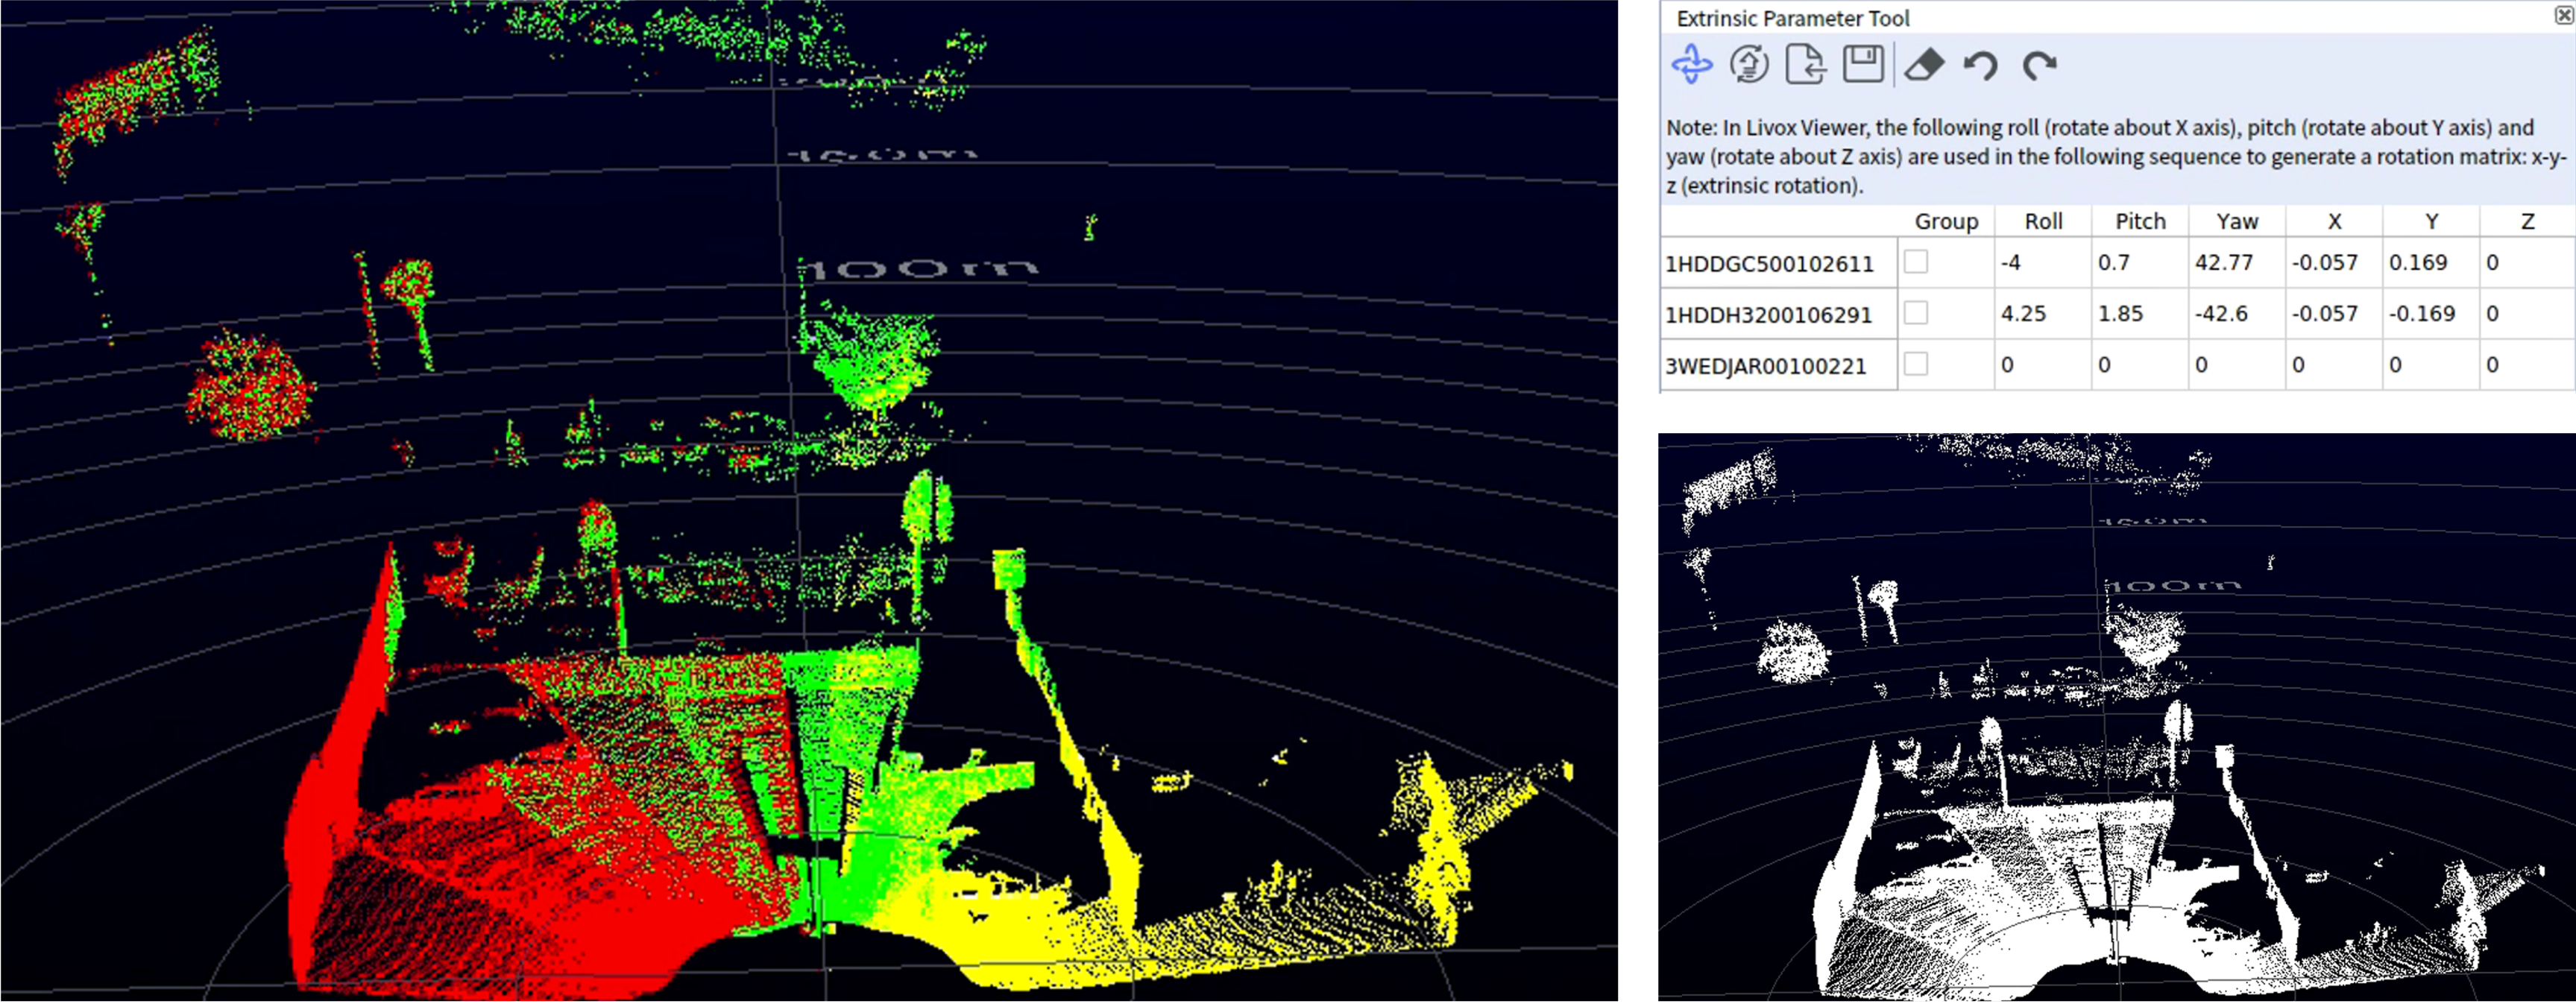
\includegraphics[width=0.95\textwidth]{Images/livox_viewer.png} 
\caption{Data from port (red), center (green), and starboard (yellow) Livox Units as viewed within the Livox Viewer software (left), and the integrated calibration tool with estimated extrinsic parameters shown (right). }
\label{fig:LidarLidar_calib}
\end{figure}

% \textcolor{red}{Insert Image from Livox Viewer Showing alignment}
%%%%%%%%%%%%%%%%%%%%%%%%%%%%
\subsubsection{Camera Calibration} \label{sec:camera_intriniscs_results}

Camera calibration was performed using a newly fabricated checkerboard target, shown in Figures~\ref{fig:checkerboard_old} and~\ref{fig:checkerboard_new}.  
The target consists of a 6$\times$9 grid of 100~mm squares, providing 40 corner features for registration.  
Thirty HDR images were captured with the checkerboard placed at positions spanning the horizontal field of view and distances between five and 40~m.
These images were then processed with MATLAB Camera Calibration app \cite{matlab_calibration}, which was successful in detecting the checkerboard in 23 separate frames.  
This initial process provided a set of camera intrinsic values with a mean pixel error of 0.63~pixels (Figure~\ref{fig:HDR_calib_error}).

\begin{figure}[htbp]
    \centering
    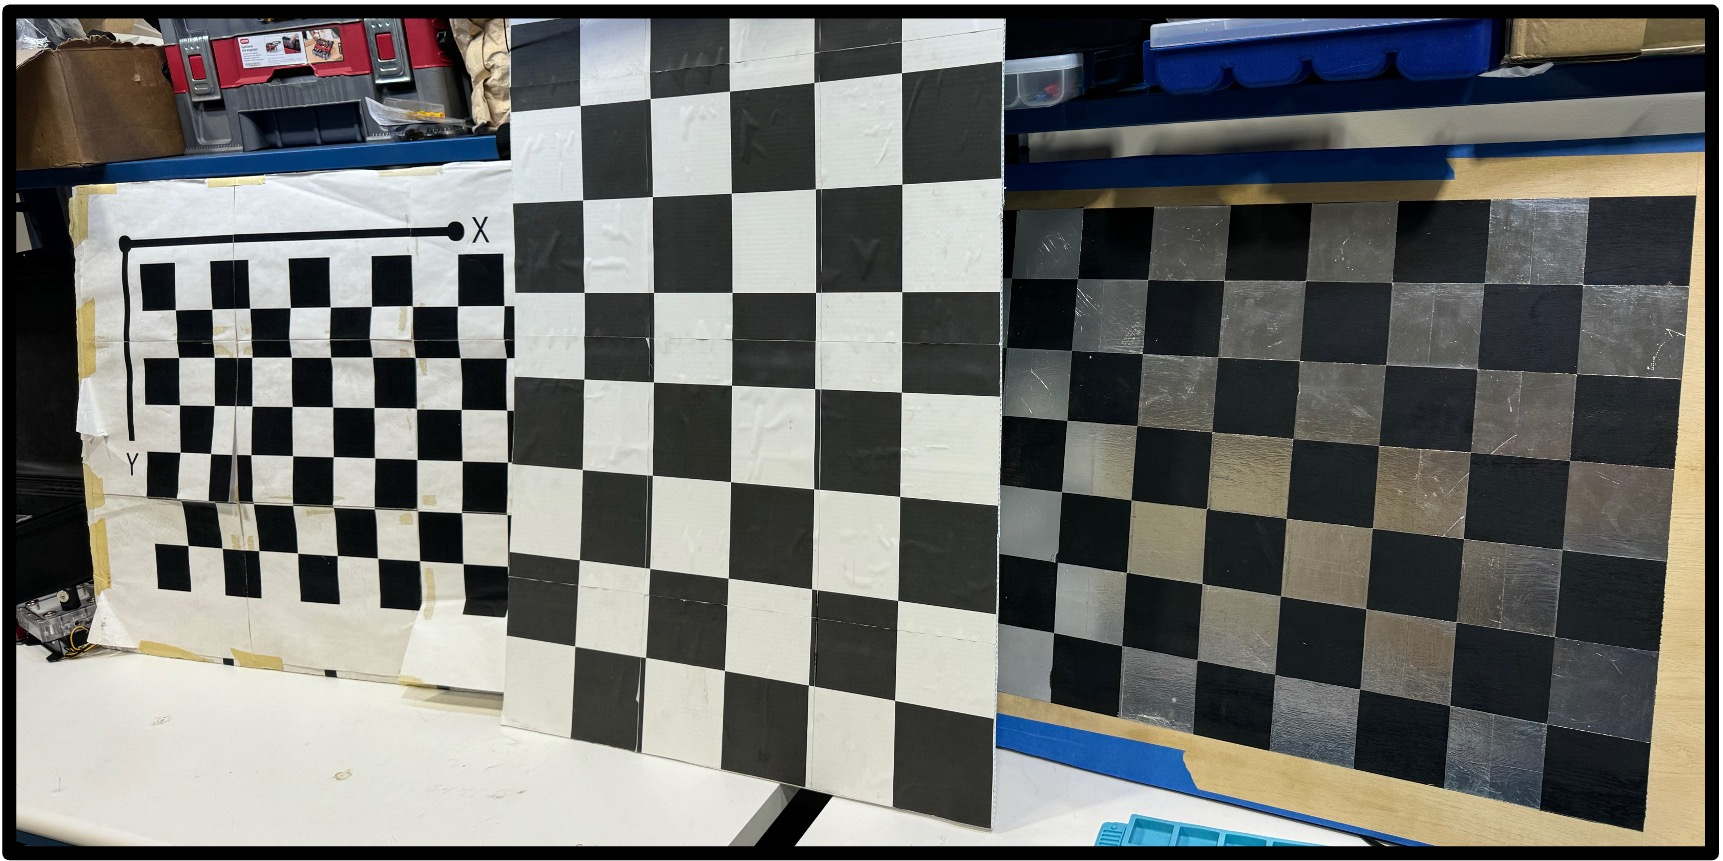
\includegraphics[width=0.9\linewidth]{Images/checkerboard_old.jpg}
    \caption{Older paper-based checkerboards maintained dimensional accuracy but degraded over time.}
    \label{fig:checkerboard_old}
\end{figure}

\begin{figure}[htbp]
    \centering
    \includegraphics[width=0.9\linewidth]{Images/Checkerboard_new.png}
    \caption{New precision-painted checkerboard target used for intrinsic calibration.}
    \label{fig:checkerboard_new}
\end{figure}

\begin{figure}[htbp]
    \centering
    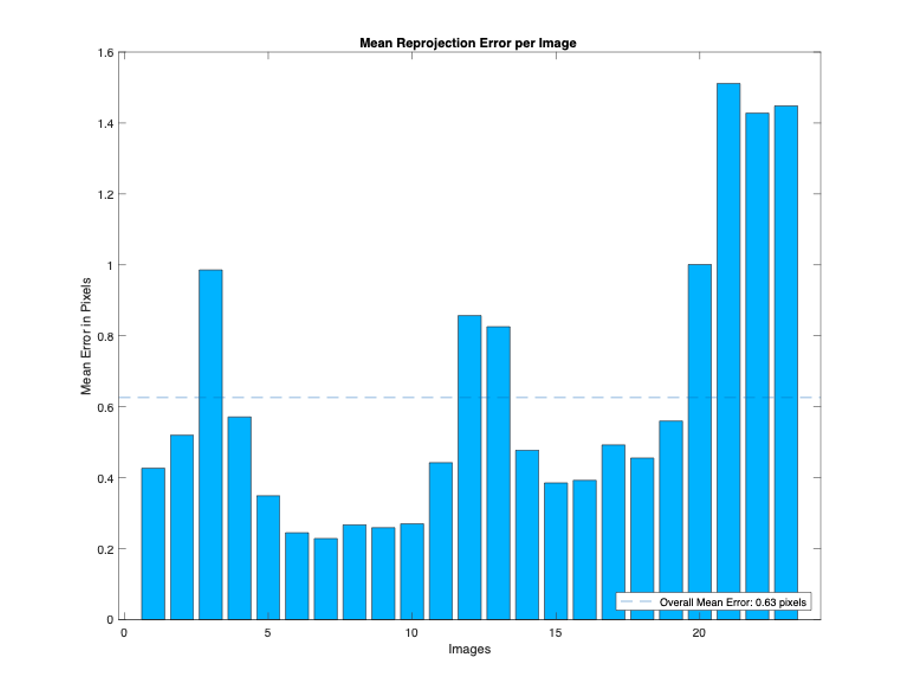
\includegraphics[width=0.9\linewidth]{Images/HDR_calib_error.png}
    \caption{Initial HDR camera calibration yielded a mean re-projection error of 0.63~pixels across the dataset.\textcolor{red}{reproduce graphic with larger text and landscape orientation. no need for square aspect ratio.}}
    \label{fig:HDR_calib_error}
\end{figure}

% The resulting transformation achieved sub-degree rotational and centimeter-level translational accuracy, sufficient for reliable fusion and object detection.
%%%%%%%%%%%%%%%%%%%%%%%%%%%%
\subsubsection{Camera–LiDAR Calibration} \label{sec:camera-lidar_results}

During extrinsic calibration, the same checkerboard images were concurrently scanned by the LiDAR.  
Each frame was held stationary while the LiDAR accumulated data over 0.5 seconds, producing a dense point cloud of the target even at ranges up to 12~m.  
These data were segmented into \acp{ROI}, matched to their corresponding image frames, and processed within MATLAB’s LiDAR Calibration tool \cite{matlab_calibration} to derive the initial extrinsic transformation.

\begin{figure}[htbp]
    \centering
    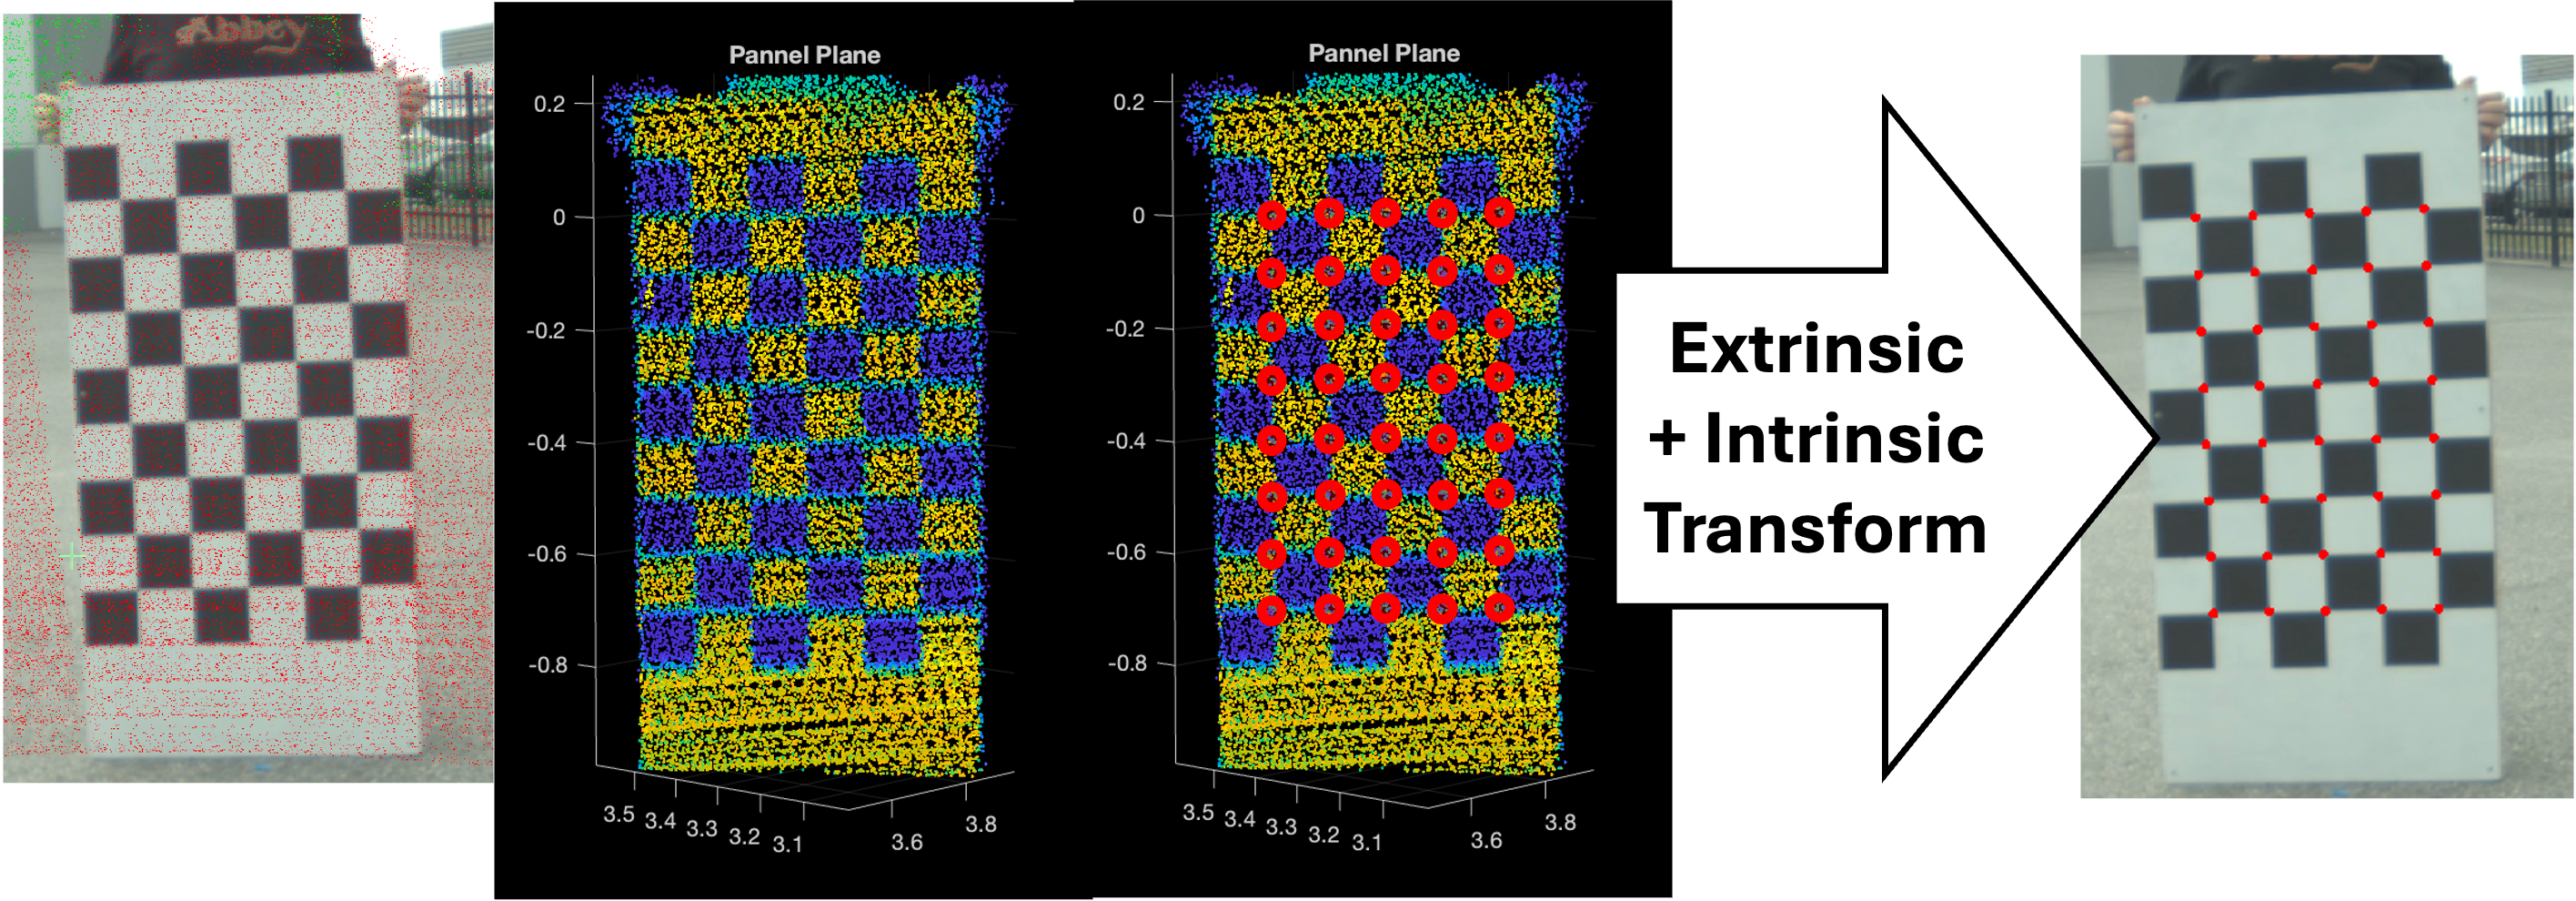
\includegraphics[width=0.8\linewidth]{Images/calib_checkers.png}
    \caption{Example of matched LiDAR point cloud and camera checkerboard detections used for extrinsic calibration.}
    \label{fig:calib_check}
\end{figure}

Subsequent manual refinement was conducted by aligning environmental features visible in both modalities, such as fences, walls, and trees, as shown in Figure~\ref{fig:LiDAR_overlay3A}.  
This process improved both extrinsic and intrinsic parameter consistency and yielded substantially higher projection fidelity.  
Comparison between early and final calibration results can be seen by comparing Figures~\ref{fig:LiDAR_overlay4} and~\ref{HDR_calib_final}.

\begin{figure}[htp]
\begin{subfigure}{\textwidth}
\centering
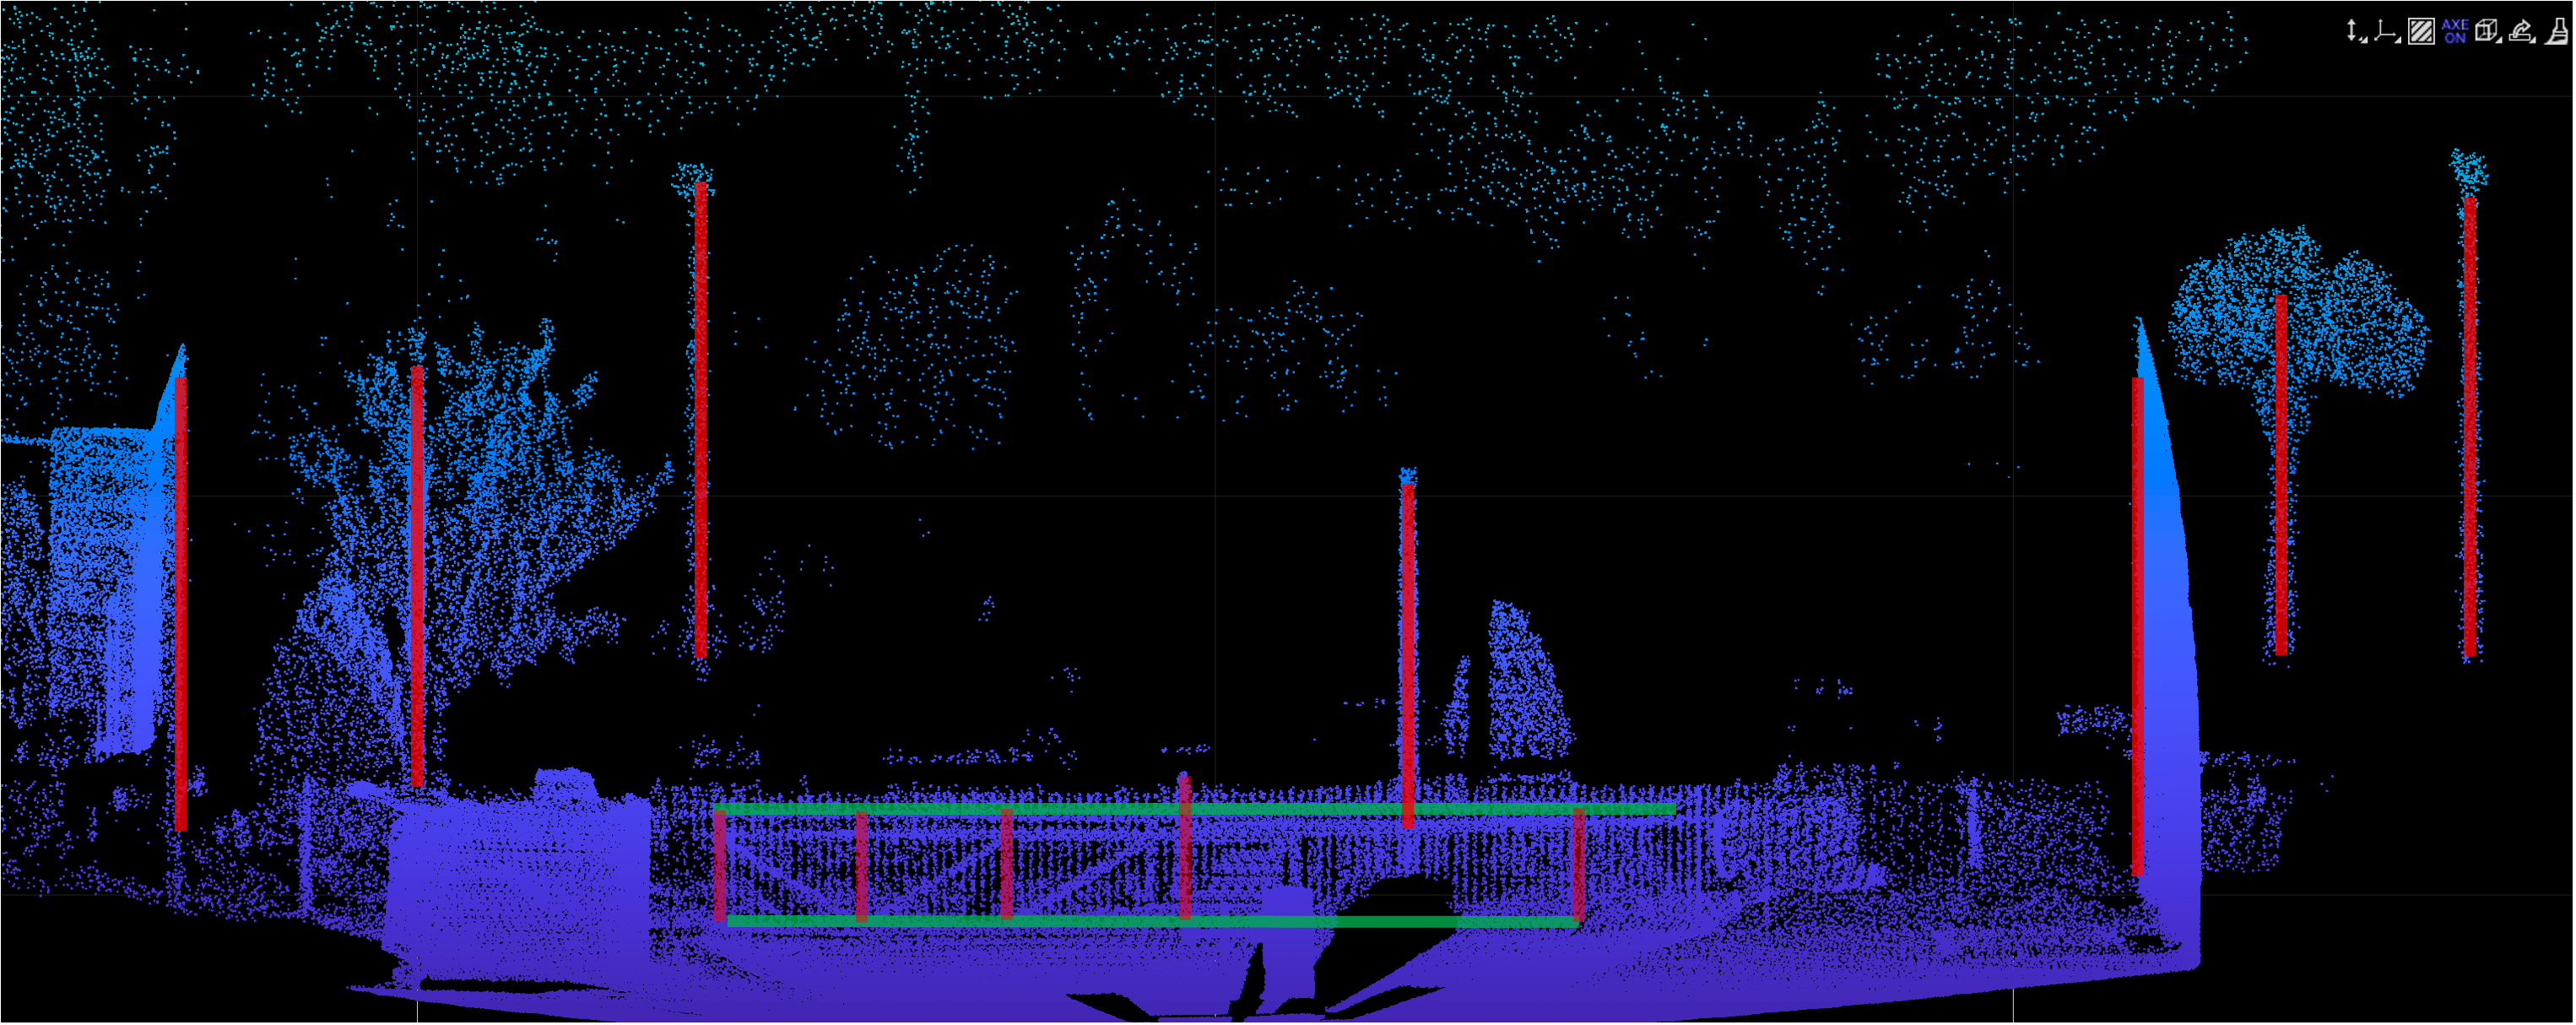
\includegraphics[width=0.94\linewidth]{Images/LiDAR_features.png}
    \caption{}
\end{subfigure}
\bigskip
\begin{subfigure}{\textwidth}
\centering
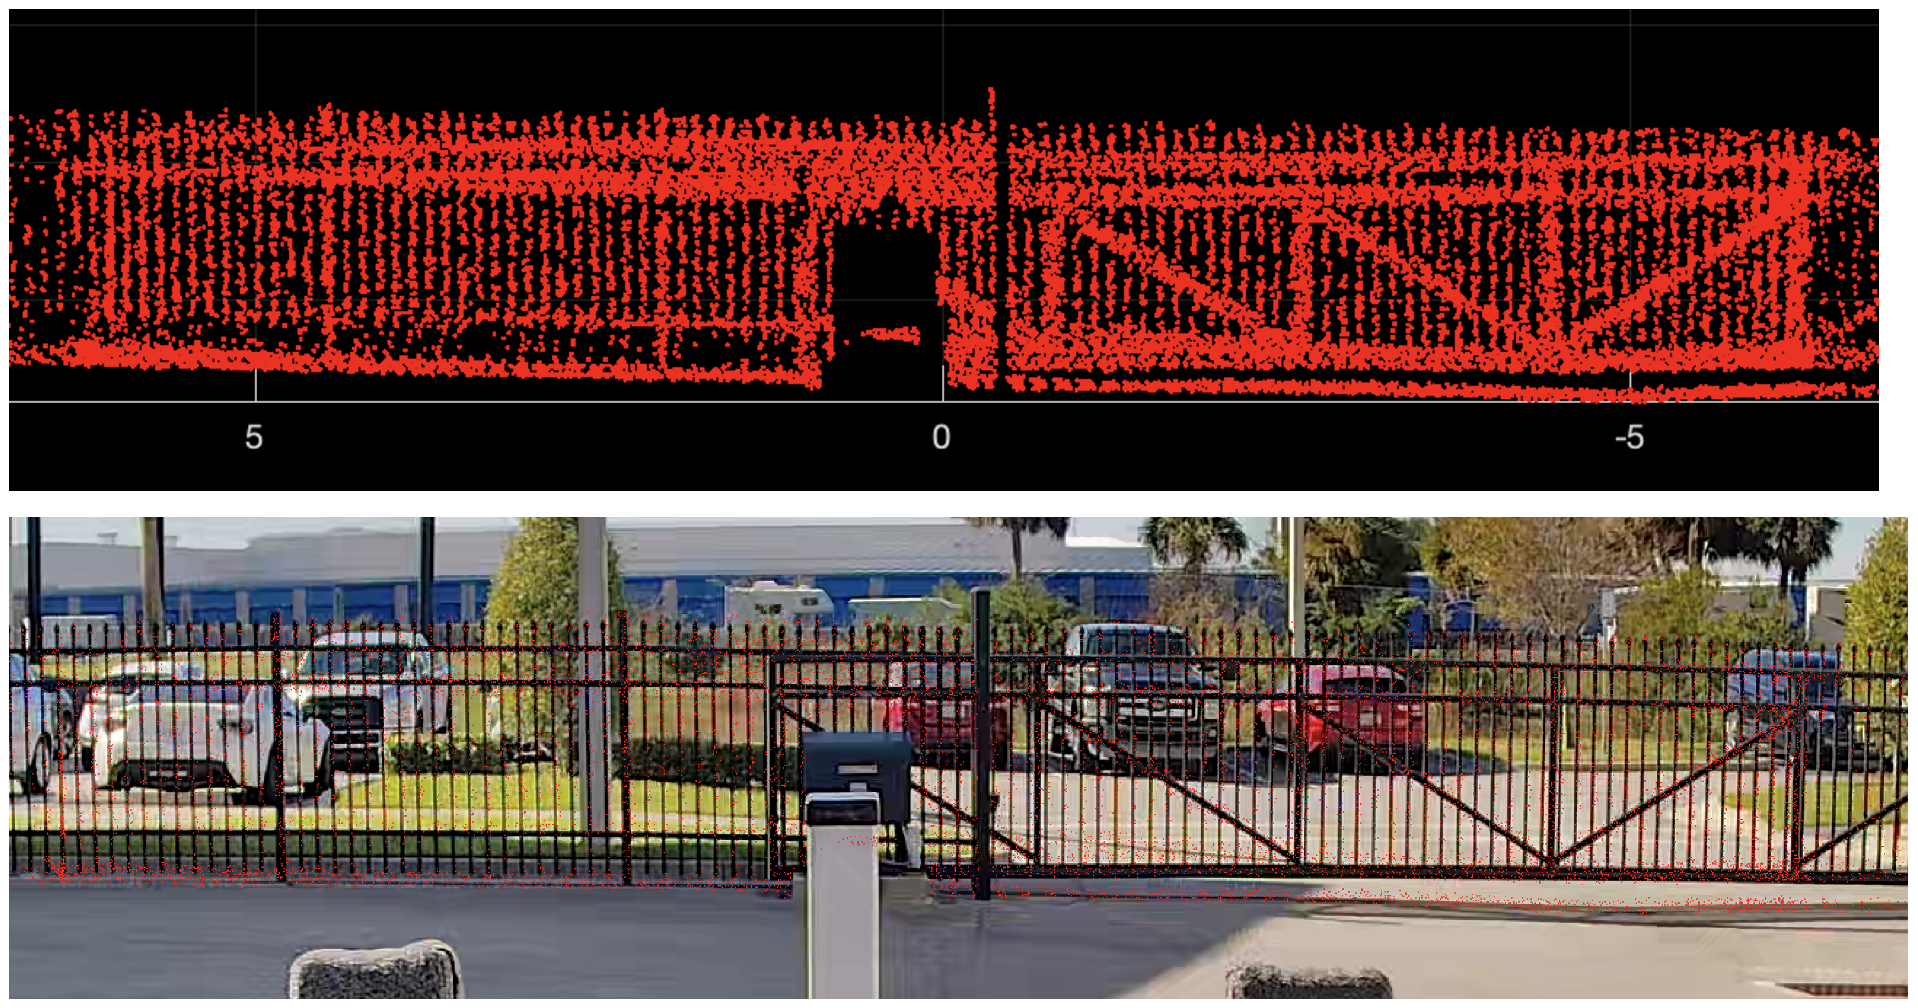
\includegraphics[width=0.94\linewidth]{Images/LiDAR_calib_fence.png}
    \caption{}
\end{subfigure}
\caption{Vertical (red) and horizontal (green) macro-level features within the point cloud (a) are isolated (b) to support visual refinement of the camera–LiDAR alignment.}
\end{figure}

\begin{figure}[ht]
    \centering
    \includegraphics[width=0.8\linewidth]{Images/LiDAR_overlay4.png}
    \caption{Initial calibration result showing early ROI-based alignment with overlaid geometric guides for evaluation.}
    \label{fig:LiDAR_overlay4}
\end{figure}
\begin{figure}[htp]
\begin{subfigure}{\textwidth}
\centering
\includegraphics[width=0.94\linewidth]{Images/LiDAR_overlay3A.png}
    \caption{Three isolated regions of interest (ROI) in the LiDAR point cloud.}
    \label{fig:LiDAR_overlay3A}
\end{subfigure}
\bigskip
\begin{subfigure}{\textwidth}
\centering
\includegraphics[width=0.94\linewidth]{Images/LiDAR_overlay3B.png}
    \caption{}
    \label{fig:LiDAR_overlay3B.png}
\end{subfigure}
\caption{Final camera–LiDAR calibration. LiDAR ROIs containing identifiable geometry (a) are projected as red pixels onto the HDR image (b) to confirm alignment quality.}
\label{HDR_calib_final}
\end{figure}
%%%%%%%%%%%%%%%%%%%%%%%%%%%%%%%%%%%%%%%%%%%%%%%%%%%%%%%%%%%%%%%%%%%%
\subsection{Temporal Calibration}
\label{time_sync}

This section discusses how each of the distributed computers and sensor are kept in sync with each other.
% Section \ref{comp:network} discussed the network architecture onboard the Minion \ac{USV} and dealt with the concept of network latency.
Section \ref{time_sync_lan} discusses how a master clock time from the GPS is distributed throughout the network, and section \ref{time_sync_cam} discusses how camera data is transferred from one machine to another without loss of timing information.
It is important to note that the temporal offsets discussed here should not be affected by the network latency described in Section~\ref{comp:network}, as timing information is transmitted with the data, and not subject to how long it takes to be delivered. 

% Latency is used to describe the discrepancy between two system clocks as well as the delay experienced in data transmission over the \ac{LAN}.
% Offset is used to discuss the difference in time between sensor data timestamps.

% an offset between system clocks, referred to here as latency, and a discrepancy between the recorded timestamps within the camera and LiDAR sensor data 

Multi-modal sensor fusion for object detection fundamentally requires precise temporal alignment between sensors operating on independent clocks and sampling at different rates.  
For example, if two sensors are offset by 200 milliseconds while observing a vessel moving at $5~\mathrm{m/s}$ and located 30~m from the platform, their detections would appear approximately $1~\mathrm{m}$ apart—equivalent to nearly $2^{\circ}$ of angular separation in the field of view.  
Such a discrepancy disrupts the spatial alignment between LiDAR points and image features, emphasizing the importance of consistent timing across all data streams.
While an inter-sensor offset of 20 milliseconds or less would ensure that collected data is within the tolerance of our detection system in a real-world scenario, this level of precision was determined to be unnecessary for the RobotX competition and was relaxed to 100 milliseconds.

% In maritime applications, where vehicle motion is relatively slow compared to ground-based platforms, sub-millisecond synchronization is generally unnecessary.  
% For the same vessel traveling at $5~\mathrm{m/s}$ and 30~m range, a temporal offset of $20~\mathrm{ms}$ limits apparent displacement to about 0.1~m, corresponding to less than two pixels in the downsampled image used for YOLO-based detection.  
% As demonstrated in Chapter~\ref{realtime_object_detection}, this level of alignment provides sufficient temporal accuracy for late-fusion operations.
% Therefore, a 20~ms offset is adopted as the maximum allowable synchronization error for this system.
% In this work, the design requirement is an inter-sensor clock \emph{offset} of $\leq 20~\mathrm{ms}$, which limits apparent target displacement to $\approx 0.1~\mathrm{m}$ at 30~m for a vessel moving at $5~\mathrm{m/s}$.  
% Note that offset (clock difference between devices) is distinct from end-to-end video latency (capture→decode delay); latency does not break fusion when frame timestamps are preserved.

% The next subsections describe the timing architecture: network synchronization across the vessel, Network Time Protocol for millisecond alignment of compute nodes, Precision Time Protocol for microsecond alignment of LiDAR units, and camera synchronization with timestamps embedded in the video bitstream and recovered at the receiver. Final timing performance and any corrective alignment used for LiDAR fusion are reported in Sec.~\ref{sec:time_sync_results}.


% Offset is the difference between device clocks at the same instant in time. 
% It shifts timestamps and creates apparent motion between modalities. 
% Latency is the delay from image exposure to availability at the receiver. Latency changes throughput but not the recorded capture time when timestamps are preserved. 
% At 5~m/s and 30~m range, a 20~milliseconds offset yields about 0.1~m apparent displacement, which is acceptable for late fusion. 
% The next subsections describe network synchronization, NTP for millisecond alignment of compute nodes, PTP for microsecond alignment of LiDAR units, and camera time-stamping within the video bitstream. Final offset and pipeline latency measurements appear in Section ~\ref{time_sync}.
% \textcolor{red}{This needs revision. The next section discusses latency, which needs to be identified as a separate measure from offset. Redo this last paragraph to correct.}

%%%%%%%%%%%%%%%%%%%%%%%%%%%%
\subsubsection{Network Synchronization} \label{time_sync_lan}

The Minion platform employs a hierarchical time synchronization architecture that distributes GPS-disciplined time from the PinPoint receiver to all perception sensors.
% \textcolor{blue}{achieving millisecond-level accuracy for camera observations and microsecond-level synchronization for LiDAR measurements. } 
In this configuration, the GPS clock serves as the master time source, which is distributed over the network via \ac{NTP} for coarse alignment or \ac{PTP} to achieve higher precision.
Together, these layers establish a unified temporal framework supporting reliable cross-modal data fusion and performance evaluation.

The synchronization hierarchy cascades timing information from the PinPoint GPS receiver, through the Atlas computing cluster, to the Jetson Xavier in the camera enclosure, and finally to each Livox Horizon LiDAR unit. This hierarchy is intentionally structured to align with the system’s physical and logical topology:

% PinPoint GPS → Atlas PC (Chrony NTP server) → Jetson Xavier (NTP client, PTP master) → Livox Horizon LiDAR (PTP clients)

At the top of this chain, the PinPoint GPS module provides Coordinated Universal Time (UTC) with sub-microsecond accuracy using the Global Navigation Satellite System (GNSS) signal. This external clock acts as the authoritative reference for the entire vessel, ensuring that all downstream systems inherit a consistent time base independent of internet connectivity.

%%%%%%%%%%%%%%%%%%%%%%%%%%%%
% \subsubsection{Network Time Protocol} \label{NTP}
% \paragraph{NTP}
Within the local area network (LAN), the Chrony \ac{NTP} daemon runs on the primary Atlas computer, which serves as the authoritative time server for all onboard devices. Chrony continuously disciplines the system clock using the GPS reference and corrects for minor drift caused by oscillator instability.

The NVIDIA Jetson AGX Xavier inside the camera enclosure operates as an \ac{NTP} client, synchronizing its system clock with the Atlas PC over the local Ethernet link. The resulting clock alignment achieves approximately 1–10~milliseconds accuracy—sufficient for coordinating 10~Hz camera streams and maintaining consistent ROS timestamps across computing nodes.

The synchronization status is verified at startup by onboard scripts that query Chrony before any video or LiDAR processes begin. This verification ensures that recording never proceeds with unsynchronized clocks. In addition, automated diagnostic checks allow operators to confirm that time distribution remains stable throughout offshore missions, where the GPS link represents the sole external time authority

%%%%%%%%%%%%%%%%%%%%%%%%%%%%
% \subsubsection{Precision Time Protocol} \label{PTP}
% \paragraph{PTP}
While \ac{NTP} provides millisecond-level precision for cameras and computing nodes, LiDAR sensors demand tighter synchronization. Each Livox Horizon operates at 100~Hz with microsecond-timestamped measurements, where even millisecond-level drift would cause measurable spatial distortion during vessel motion. To meet this requirement, the Jetson Xavier distributes the \ac{PTP} signal using the Linux ptp4l service.

In this configuration, the Jetson acts as the \ac{PTP} master clock, broadcasting timing packets over the camera-enclosure network to all three Livox devices, which function as \ac{PTP} slaves. \ac{PTP} uses hardware-timestamped Ethernet packets to measure network delay symmetrically and correct for it in real time, achieving sub-microsecond synchronization between LiDAR units. The Livox Viewer utility confirms synchronization state during system startup, and visual indicators within the GUI report “active 1588 signal” once synchronization is established.

\begin{figure}[htbp]
\centering
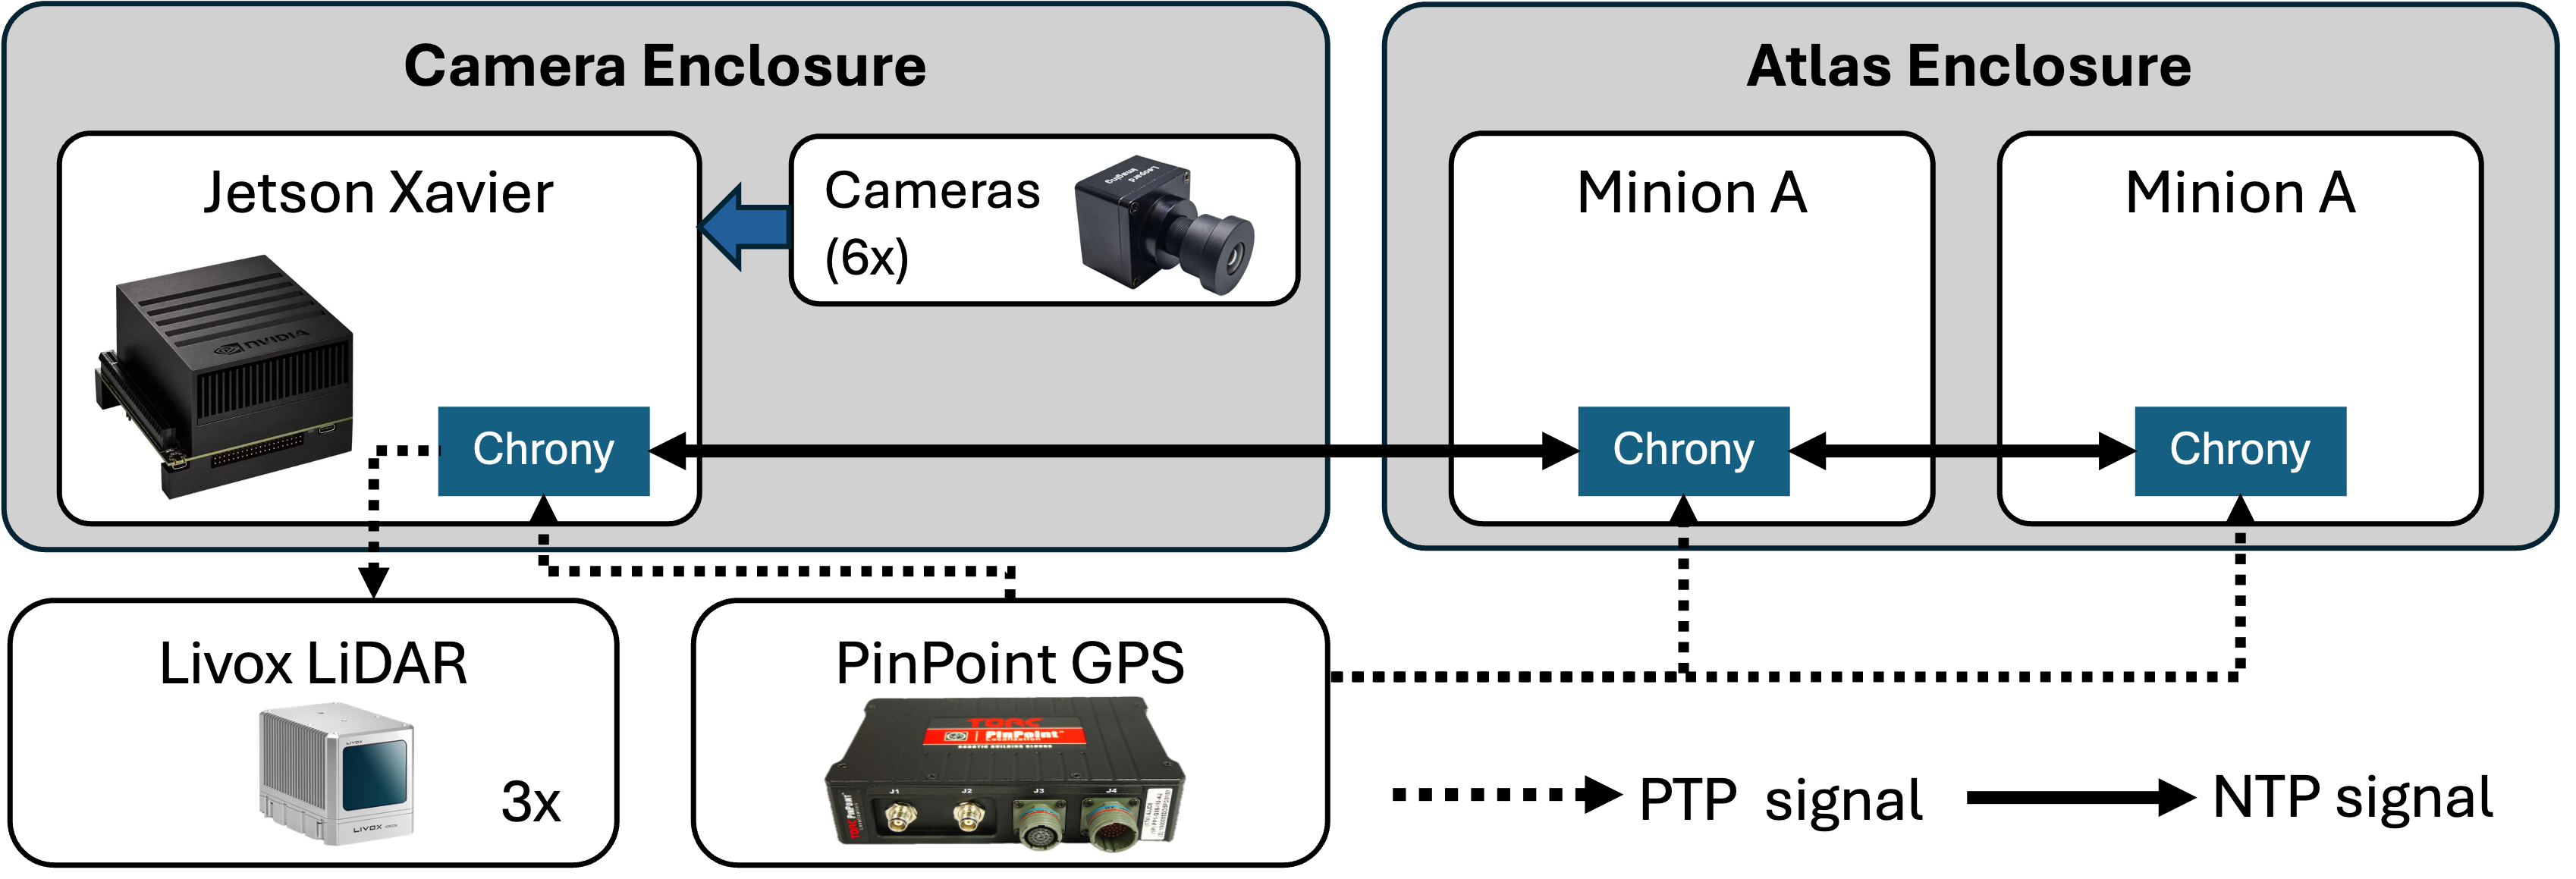
\includegraphics[width=0.8\textwidth]{Images/NTP.png}
\caption{LAN diagram for Minion USV}
\label{fig:network_sync}
\end{figure}

%%%%%%%%%%%%%%%%%%%%%%%%%%%%%%%%%%%%%%%%%%%%%%%%%%%%%%%%%%%%%%%%%%%%
\subsubsection{Camera Synchronization} \label{time_sync_cam}

Accurate video timestamps are essential for aligning image data with LiDAR point clouds. To achieve frame-level temporal precision, the Minion system embeds timestamps directly into the H.264/H.265 video stream generated by the Jetson Xavier using the GStreamer framework. This ensures that timing information remains synchronized with the frame itself, surviving compression, transmission, and playback.

% \paragraph{prior solution}
% Earlier implementations of the Minion perception system—originally developed by Thompson~\cite{thompson2023} employed a custom GStreamer plugin that performed two timestamping operations.
% First, it generated an adjacent .csv file containing timestamps that aligned to each frame of locally recorded video; second, it embedded the same timestamps into the closed-caption (CEA-608) layer of the \ac{RTSP} video stream.
% While this method was effective for offline data processing using the locally saved video files, the video stream is conducted asynchronously, and the RTSP protocol is unable to keep the closed-caption stream data linked to video frames.
% This limitation motivated the development of an \ac{SEI}-based synchronization method described below.
Earlier implementations of the Minion perception system—originally developed by Thompson~\cite{thompson2023}—employed a custom GStreamer plugin that performed two time-stamping operations. 
First, it generated an adjacent .csv file containing timestamps aligned to each frame of the locally recorded video. 
Second, it embedded the same timestamps into the closed-caption (CEA-608) layer of the \ac{RTSP} video stream. 
While effective for offline data processing using the saved video files, this method was limited by the asynchronous nature of \ac{RTSP}, which cannot maintain a persistent link between closed-caption data and video frames. 
This limitation motivated the development of the \ac{SEI}-based synchronization method described below.

% \paragraph{developed solution}

The current implementation replaces the caption-based approach with direct timestamp embedding using Supplemental Enhancement Information (SEI) Network Abstraction Layer (NAL) units defined in the H.264/H.265 standard.
Each video frame receives a GPS-disciplined system timestamp at the instant of capture from the camera sensor. These timestamps are stored as 64-bit values (milliseconds since Unix epoch) and attached to each frame via a custom GStreamer extension. % (CustomTimestampMeta).
This method keeps the timestamp data inextricably linked to the same video layer that is transmitted over \ac{RTSP}, guaranteeing that each video frame received will have a timestamp, even if dropped frames are experienced.
The complete video processing pipeline is visualized as a block diagram in Figure \ref{video_pipeline}.

% During encoding, a pad probe inserts the SEI NAL units immediately before the RTP payload (rtph264pay), ensuring that every encoded frame carries its own timestamp embedded within the bitstream.
% Because this method fits within the encoding standard, the timestamps persist through compression and streaming, which eliminates the complexity of the prior approach and maintains compatibility with all conventional video decoders.

\begin{figure}[htbp]
\centering
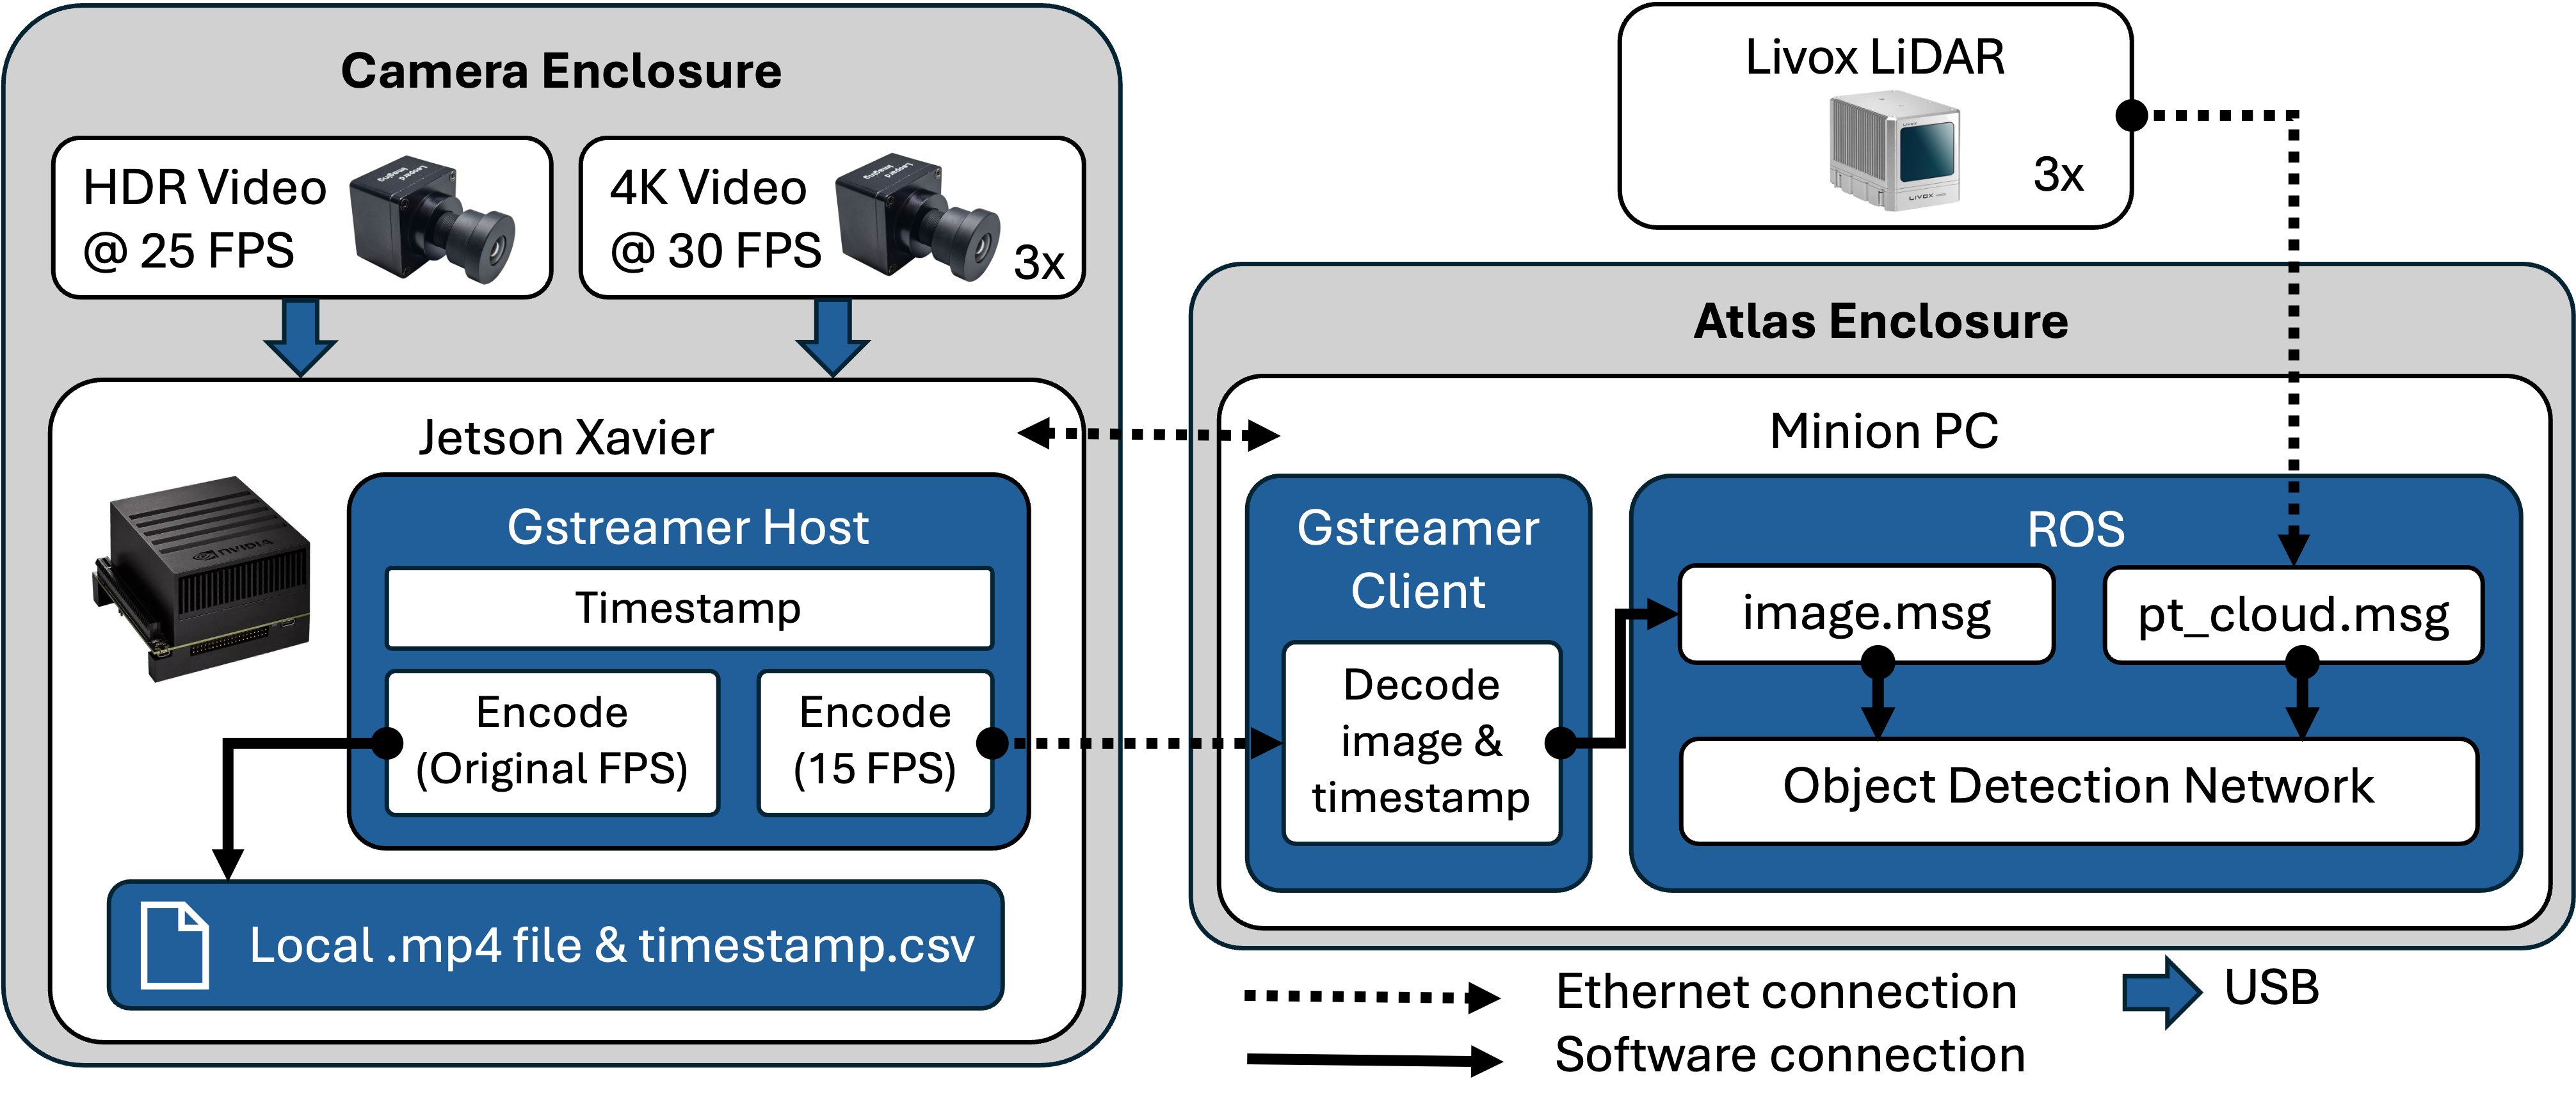
\includegraphics[width=0.8\textwidth]{Images/Block_Diagram.png}
\caption{LAN diagram for Minion USV}
\label{fig:sensor_block_diagram}
\end{figure}



% v4l2src → videoconvert → videorate → x264enc → [SEI insertion] → rtph264pay → RTSP stream

% Captured video at 2880×1860px and 60fps is downsampled to 10fps for transmission, balancing temporal resolution with network bandwidth. The SEI timestamp metadata is attached prior to frame-rate conversion, ensuring that each output frame retains its original capture time.
% The pipeline is fully compliant with ITU-TH.264 Annex~D and has been verified for compatibility with both H.264 and H.265 encoders.

At the receiving end, the Atlas PC decodes incoming streams using a complementary GStreamer pipeline equipped with a pad probe on the \texttt{h264parse} element. This probe identifies SEI NAL units and extracts the embedded timestamp payload before decoding. The recovered timestamps are then written to the ROS message headers of the corresponding image frames via the \texttt{image\_transport} framework.


\begin{figure}[htbp]
\centering
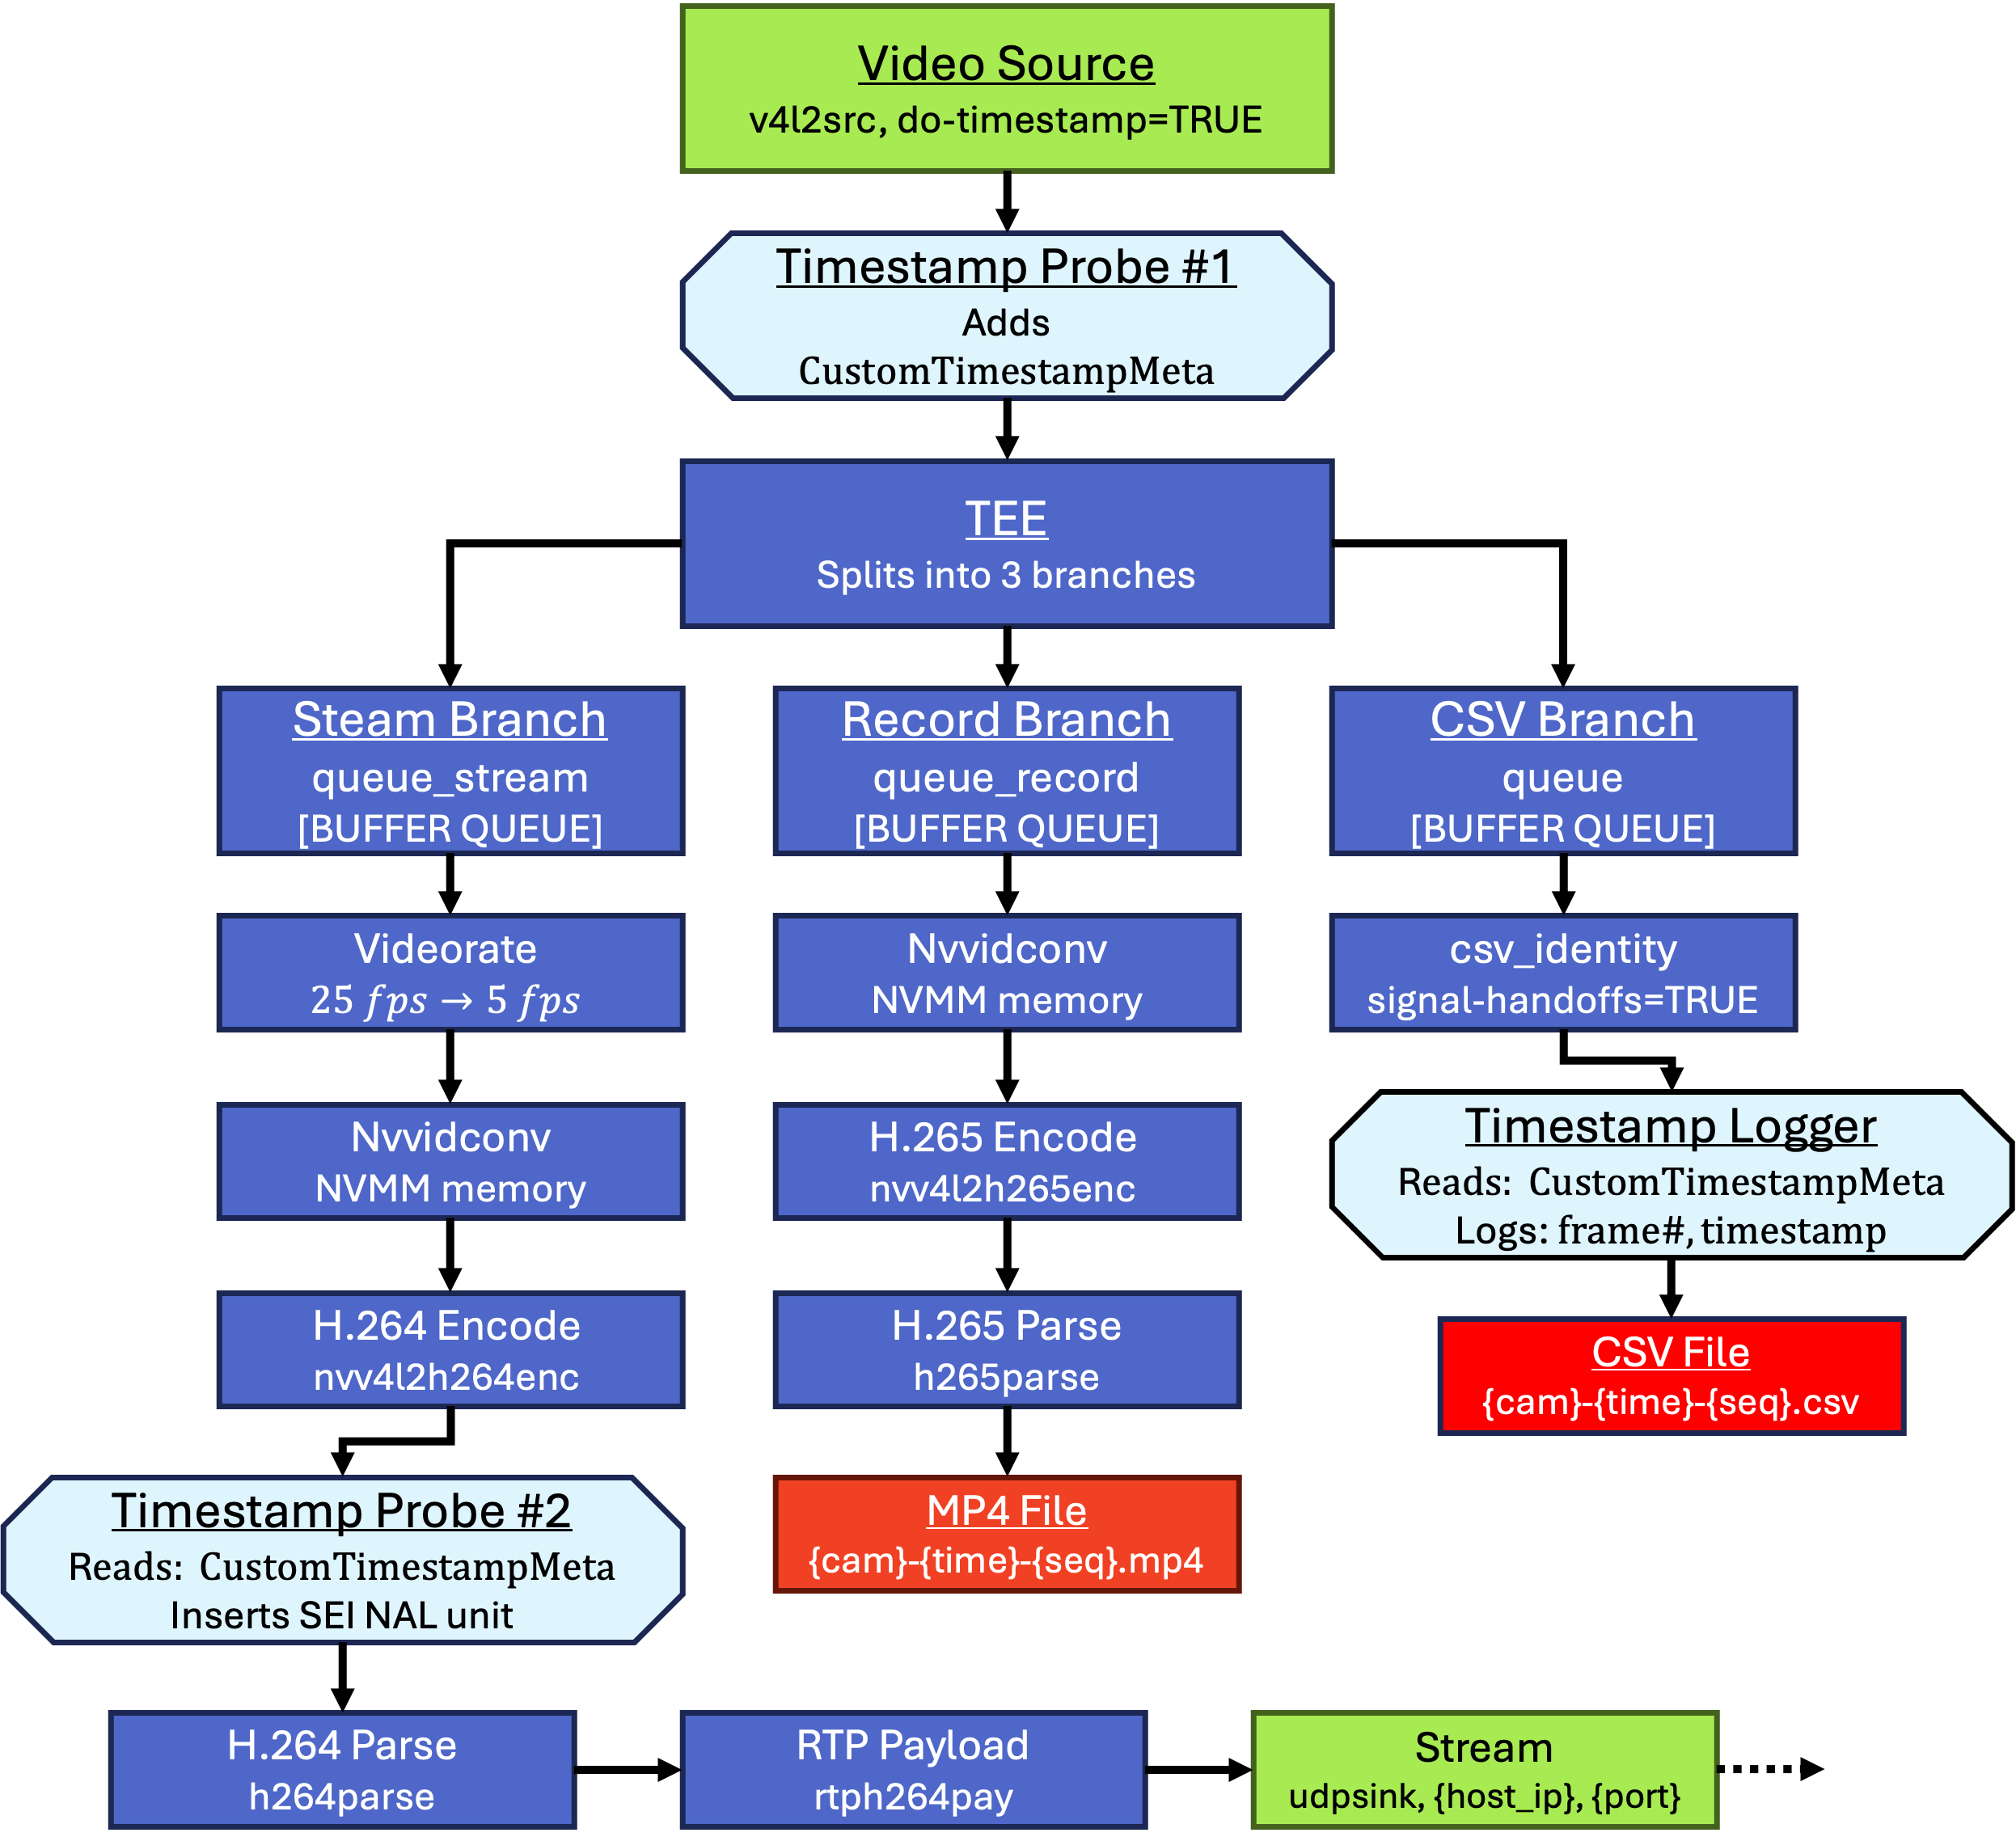
\includegraphics[width=5in]{Images/gstreamer_block.png}
\caption{Block diagram of the NVIDIA Jetson's video pipeline. Green rectangles represent video data entering or leaving the pipeline, while red rectangles indicate local file creation. Light-blue rectangles with chamfered corners denote timestamp acquisition and application operations within the pipeline.}
\label{video_pipeline}
\end{figure}
%%%%%%%%%%%%%%%%%%%%%%%%%%%%%%%%%%%%%%%%%%%%%%%%%%%%%%%%
\subsection{Results: Temporal Synchronization} \label{results)time_sync_cam}

An initial evaluation of the video stream and time-stamping system was conducted under conditions that simulated expected network load conditions.
Video data was recorded for 14.5 seconds at 10 \ac{fps} (twice the anticipated operational rate) for a total of 8,720 frames. 
The NVIDIA computer in the camera enclosure was accessed via SSH terminal and displayed a log of each timestamp being recorded and sent over the RTSP video stream. 
Similarly, the Atlas PC was connected to via SSH and displayed the timestamp being received over the RTSP video stream.
This data was also logged in a text file on the respective machines and compared for analysis. 
To ensure real-world clock precision, a real-time clock was set up in front of the camera displaying the current time, and transmitted as the subject of the video feed. An image of this setup is presented in Figure~\ref{fig:time_sync1}
This allows for any internal clock drift to easily be identified by comparing the transmitted timestamp to the time displayed in the video itself.

\begin{figure}[htbp]
    \centering
    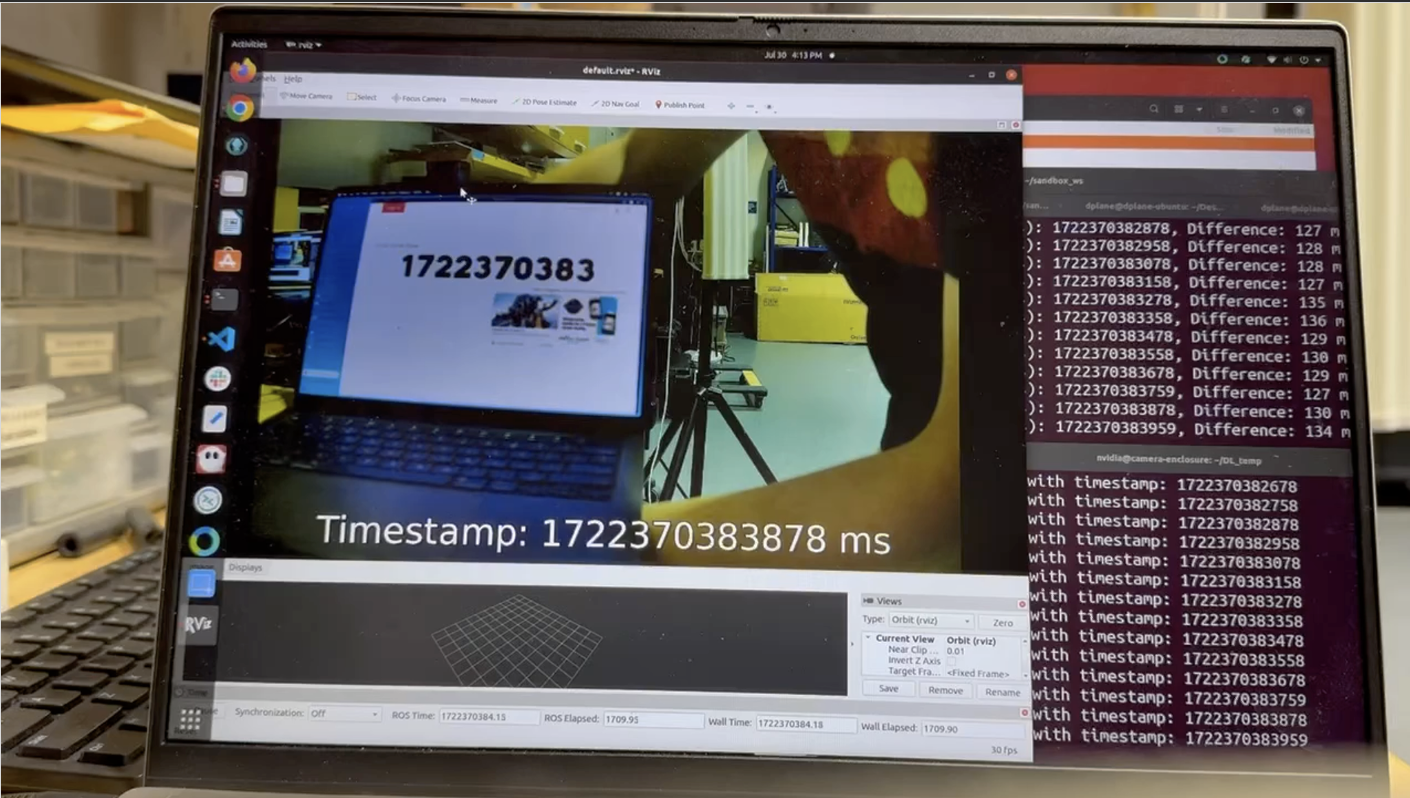
\includegraphics[width=0.8\linewidth]{Images/time_sync1.png}
    \caption{Testing the timestamp embedding within the RTSP stream for dropped frames and real-world temporal accuracy.}
    \label{fig:time_sync1}
\end{figure}
% Data was recorded by outputting the timestamps being sent and received by video camera, as well as by exporting this data to a log file on each machine. 

During the test, system-wide clock synchronization was measured using Chrony, which reported an average offset of $197;\text{ms};\pm;33;\text{ms}$ between the NVIDIA Jetson and Atlas machines.
The results of this test showed a total delay in video frame reception of 127 milliseconds, and logs between computers showed zero dropped frames with a 100\% match between timestamps.
\textcolor{blue}{This test was performed on Helios - Not Atlas, and did not have a true "master clock", if I recall. Find more recent test data. I would bet that running with updated chrony and ptp4l settings reduces this number significantly.}

Despite this result in frame delivery and timestamp assignment during testing, analysis of the recorded ROS bagfile data revealed a measurable drift between the original frame timestamps on the Jetson and those recorded by the Atlas system. 
% This discrepancy is believed to stem from thermal issues within the camera enclosure that were encountered during data collection.
% Therefore, some postprocessing of the data was required to ensure its validity.
This discrepancy is believed to result from thermal effects within the sealed camera enclosure during extended operation. 
Although no direct temperature measurements were recorded during this test, subsequent observations suggest that overheating may influence the Jetson's internal clock stability. 
This hypothesis remains unverified and will be revisited in Section~\ref{recommendations}.

To resolve this, structural similarity (SSIM) scoring was employed to match each frame recorded by ROS on the Atlas to its corresponding source frame from the original video files on the Jetson. 
Although SSIM is conventionally used to assess visual degradation from compression, in this context, it served as a frame-matching metric: matched frames produced SSIM scores near 1.0, while mismatches scored closer to 0.0. The SSIM metric used is defined as:
\begin{equation}
    \text{SSIM}(x, y) = \frac{(2\mu_x\mu_y + C_1)(2\sigma_{xy} + C_2)}{(\mu_x^2 + \mu_y^2 + C_1)(\sigma_x^2 + \sigma_y^2 + C_2)}
\end{equation}

In this expression, $\mu_x$ and $\mu_y$ represent the mean pixel intensities of images $x$ and $y$, $\sigma_x^2$ and $\sigma_y^2$ are their variances, $\sigma_{xy}$ is the covariance between the images, and $C_1$ and $C_2$ are small constants that stabilize the division when the denominator is near zero.

To initialize alignment for each bag file, the first five ROS image messages within each bag were manually paired to the corresponding frames in the source video.
This established the offset the system was experiencing at the time the data was being recorded, which was then used to programmatically pair the remaining image messages in the bag with their video frame counterparts.
SSIM-based alignment was then automated on a subset of frames sampled at one-second intervals across each bagfile. 
Once alignment was confirmed through SSIM scores, the timestamps and frame indices for the intermediate frames were interpolated from the verified matches. 
Accordingly, the total number of frames analyzed by SSIM is approximately equal to the total number of seconds of recorded data.

To streamline this process across all 112 recorded bag files, a database was created to store file names, paths, and relevant metadata, allowing image and video data to be easily cross-referenced between the video and CSV files, and more than 100,000 ROS image messages. 
The same database also served as the repository for SSIM scores, interpolated matched frame numbers, and both the original and corrected timestamps for each image message. 
This dual-purpose design enabled automation of the SSIM alignment process while simultaneously providing a complete record of the aligned frame data for offline analysis and validation.

%%%%%%%%%%%%%%%%%%%%%%%%%%%%%%%%%%%%%%%%%%%%%%%%%%%%%%%%%%%%%%%%%%%%
%%%%%%%%%%%%%%%%%%%%%%%%%%%%%%%%%%%%%%%%%%%%%%%%%%%%%%%%%%%%%%

\end{document}
